\section{Introduction}

Many everyday fluids---yogurts, pastes, sauces, slurries, cosmetic
emulsions---exhibit non-Newtonian behaviour that governs how they
pour, spread, cling, and deform. Parallel-plate and cone-and-plate
rheometers measure this behaviour through a controlled-gap shear
flow, but fail on materials with inclusions larger than the
measurement gap and on materials whose rheology evolves faster than
the lab procedure can capture.

Non-Newtonian video rheometry~\cite{hamamichi2023nonnewtonian}
addresses this gap by estimating Herschel--Bulkley parameters
from a simple dam-break flow: a material point
method (MPM) forward model is repeatedly executed inside an optimiser
until the simulated flow reproduces the observed silhouette. The
approach handles materials that instrumental rheometers cannot, but its
inner loop takes \emph{around eight hours per experimental setup}. This
latency is especially limiting for materials whose state changes during
measurement---sedimentation, ageing, temperature drift, mixing history,
or cooking cooldown---because the recovered parameter may describe a
past state rather than the current batch. Our goal is therefore not to
change the dam-break physics model, but to make the same forward
relation cheap enough for interactive inverse queries, ambiguity
diagnostics, and repeated freshness checks.

The method therefore consists of two core algorithmic components and a
validation program. We present a surrogate-accelerated framework that
reduces the inverse from hours to seconds per experimental setup: in the evaluated
implementation, a $512$-candidate inverse scoring and plausible-set
summary pass takes $3.63$\,s per case/setup, and one surrogate
candidate/setup evaluation takes $7.09$\,ms. We validate forward
fidelity, uncertainty/error calibration, ambiguous-solution reporting,
multi-observation diagnostics, speed, real-material replay, and a
held-out repeated-capture freshness protocol.
The gain is not claimed to come from a more accurate optimiser:
CMA-ES-style derivative-free search is compatible with the same
surrogate objective. The speedup comes from replacing MPM calls inside
the inverse by batched surrogate evaluations, and the reported candidate
set makes the score and retained ambiguity auditable.

\emph{(i) Local Gaussian-process (GP) forward surrogate.}
We replace repeated MPM calls by a pre-trained bank of local
Gaussian-process models. The surrogate maps
$(n,\eta,\sigma_Y,W,H)$ to the eight dam-break flow-front positions
$(x_{01},\ldots,x_{08})$ and provides both a prediction and an
uncertainty estimate for inverse estimation. The eight outputs are used
directly; we do not compress them with principal component analysis
(PCA).

\emph{(ii) Uncertainty-aware inverse reporting.}
Because a single dam-break trajectory can leave multiple plausible
Herschel--Bulkley parameters, the inverse should not always collapse
to one overconfident answer. We therefore validate both point
estimates and sets of plausible candidates, using the surrogate's
uncertainty and validation residuals to decide when ambiguity should
be reported.

\emph{(iii) Freshness-oriented repeated-measurement protocol.}
The seconds-scale inverse makes within-batch repeated captures
practical. We use two short-time setups for inverse estimation and hold
out a third setup from the same session for flow-front and binary-mask
replay. This tests repeated-capture consistency rather than fitting a
kinetic law for material ageing.
This is a validation of repeated-capture consistency, not a claim that
the paper has fitted a full kinetic law.

Hamamichi et al.~\cite{hamamichi2023nonnewtonian} established
non-Newtonian video rheometry as a viable inverse-estimation method
and identified the yield-stress/consistency degeneracy that motivates
multi-setup joint inversion. However, their simulation-in-the-loop
implementation leaves each setup as an hours-scale optimisation. Our
work inherits their dam-break protocol, observation-matching inverse,
and multi-setup formulation, but replaces repeated MPM calls with a GP
surrogate and explicit surrogate-error model. The result is the same
physical inverse problem evaluated at seconds-scale latency.
Multi-setup disambiguation and setup selection remain inherited
acquisition protocols; they are treated here rather than as a new
physical disambiguation principle.

\section{Related Work}

\subsection{Physical Measurements and Flow Rheology Signals}

Quantitative rheology is traditionally measured with rheometers
(parallel-plate, cone-and-plate, or rotational) that apply a
controlled laminar flow under known shear rate to recover the
constitutive relation between shear stress and shear rate. These
instruments require a narrow gap to enforce a clean shear profile,
which excludes materials with millimeter-scale inclusions, as well
as materials whose rheology evolves faster than the lab procedure
can capture. Less-controlled but more accessible alternatives, such
as the Bostwick consistometer, give a single readable measurement
from a simple dam-break test.

Gravity-driven flow has a long pedigree as a rheometric observation
that complements idealized-flow rheometers. The slump test
of~\citet{pashias1996fifty} recovers yield stress from a single
geometric reading; \citet{roussel2005fiftycent} extend this argument
to the spreading regime that matches dam-break geometry directly;
the final-deposit shape of a stopped free-surface flow is itself a
rheological signature~\cite{coussot1996rheological};
and~\citet{ancey2007plasticity} frames the broader class of
gravity-driven yield-stress flows as a standard rheometric regime.
The relation between flow-front position and Herschel--Bulkley
parameters is made quantitative by the similarity analyses
of~\citet{liumei1989slow} and~\citet{balmforth2007two}, the same
analytic framework used by~\citet{hamamichi2023nonnewtonian} to
explain when different Herschel--Bulkley triples produce similar
dam-break trajectories.

Our forward simulator inherits the MPM lineage brought into
graphics by~\cite{stomakhin2013material,jiang2015affine,hu2018moving,
jiang2016material}, with yield-stress rheology realised through
return-mapping
formulations~\cite{yue2015continuum,ram2015material,klar2016drucker,
tampubolon2017multi,wolper2019cdmpm}. We use the Herschel--Bulkley
return map of~\citet{yue2015continuum} on
Taichi~\cite{hu2019taichi}; \citet{nagasawa2019mixing}, from the
same lab as our predecessor, shares our material focus.


\subsection{Video-Based Material Estimation}

Estimating simulation parameters from video by matching rendered and
observed dynamics has a long lineage in graphics and
vision~\cite{bhat2002computing,monszpart2016smash}.
\citet{takahashi2019video} established the video-to-parameter pattern
for viscous fluids by matching rendered and observed dam-break
silhouettes per scene; \citet{hamamichi2023nonnewtonian} extended
this to the Herschel--Bulkley triple $(n,\eta,\sigma_Y)$ and is the
direct predecessor of our work. We inherit their dam-break observation
protocol, parameterisation, and multi-setup formulation for resolving
the yield-stress/consistency degeneracy. The difference is
computational rather than physical: their inverse repeatedly calls
MPM inside the optimiser, whereas ours evaluates the same forward
relation through a trained GP surrogate and reports the remaining
ambiguity explicitly.

Related work recovers material parameters from other visual
modalities: video-based cloth friction~\cite{rasheed2020visual},
particle-image-velocimetry-based rheology through physics-informed
networks~\cite{thakur2025learning}, and consumer-video neural
regression for scalar viscosity~\cite{rauzan2024protorheology}. These
target different material classes or observation modalities and do
not provide the same dam-break video inverse for
$(n,\eta,\sigma_Y)$. Free-surface extraction from experimental video
is treated in~\cite{cochard2009tracking}. Inverse rheometry has also
been approached for pseudoplastic gravity-driven free-surface flows
using adjoint-based inverse models~\cite{martin2015inverse}; our
setting instead uses a three-dimensional MPM dam-break simulator as
the reference forward model and amortises its online cost with a
GP surrogate.

An alternative paradigm pursues parameter recovery via differentiable
simulation. The differentiable MLS-MPM
family~\cite{hu2019chainqueen,hu2020difftaichi,huang2021plasticinelab}
has been applied to deformable and plastic materials;
gradSim~\cite{murthy2021gradsim} demonstrates end-to-end
differentiable physics with differentiable rendering. Most relevant
to non-Newtonian recovery from video,
PAC-NeRF~\cite{li2023pacnerf} couples differentiable MPM with NeRF
rendering to recover viscosity parameters from multi-view video, and
Eastman~\cite{eastman2024recovery} recovers Herschel--Bulkley
parameters from a ketchup column-collapse video via differentiable
MPM and neural rendering. These approaches optimise through a
scene-specific differentiable computation graph. Our aim is
complementary: we precompute a reusable probabilistic emulator for a
fixed dam-break protocol, so that many inverse queries can be run
without a new MPM solve or a new differentiable optimisation for each
video.


\subsection{Identifiability and Multi-Setup Disambiguation}

Free-surface motion can contain substantial rheological information,
but the amount available depends on what part of the free surface is
observed and how it is summarised. \citet{martinpritchard2022inferring}
show that a generalized Newtonian constitutive function can be
identified from free-surface evolution under their model assumptions;
\citet{ahmadi2022identification} analyse the sensitivity of
Herschel--Bulkley parameters to free-surface measurements; and
\citet{muchiri2024identification} recover yield stress and
consistency from shallow-water elevation hydrographs under
viscoplastic rheology. These results motivate free-surface inverse
rheometry, but they do not remove the practical degeneracy created by
our lower-dimensional observation, the eight flow-front positions
$(x_{01},\ldots,x_{08})$.

For the dam-break protocol used here, \citet{hamamichi2023nonnewtonian}
identify a yield-stress/consistency ridge and propose sequential
multi-setup inversion to reduce it. We retain this interpretation:
additional setups are evidence for disambiguation, not a guarantee
that a single observation has a unique parameter triple. In the
surrogate setting, this issue becomes a validation question. A good
inverse should show that the set of physically plausible parameter
candidates shrinks across setups while preserving the correct basin
on synthetic tests, and should avoid presenting a single point
estimate when the observed trajectory does not justify one.


\subsection{Surrogate-Accelerated Inverse}

Gaussian-process regression~\cite{rasmussen2006gaussian} pairs
flexible nonparametric regression with calibrated predictive
uncertainty, making it a natural surrogate for expensive simulators.
Local or expert-based GP models~\cite{jordan1994hierarchical,
tresp2001mixtures,liu2018generalized} use specialist regressors to
handle heterogeneous data; our bank follows this local-emulator
principle but routes by dam-break geometry and trajectory shape rather
than by a learned global gate.

Inverting expensive simulators has been studied under Bayesian
calibration of computer models~\cite{kennedy2001bayesian} and
computer-model validation~\cite{bayarri2007framework}; Bayesian
optimisation~\cite{snoek2012practical,shahriari2016taking} and
CMA-ES~\cite{hansen2016cma} are common search layers. We therefore keep
the search mechanism secondary: CMA-ES can be run over our GP/BAE score,
but the central question in this paper is not which optimiser finds a
low score, but whether that score is trustworthy and whether ambiguity
is retained when the observation is underdetermined.

The substitution itself must be validated rather than assumed.
\citet{stuart2018posterior} bound the Hellinger distance between
surrogate-based and true-simulator posteriors by moments of the
surrogate's predictive error, with the bound extended to
learned-hyperparameter settings by~\citet{teckentrup2020convergence}.
Our implementation follows the same principle at the level of
engineering diagnostics: the inverse objective uses the GP predictive
variance together with validation residual variance and observation
noise. The experiments therefore report not only the best selected
parameter estimate, but also whether the plausible candidate set still
contains the correct basin.
The same caution applies to setup proposal: optimal experimental
design (OED) for nonlinear inverse problems is commonly formulated
through posterior uncertainty or information gain~\cite{chaloner1995bayesian},
and recent work
builds Bayesian approximation error (BAE) terms directly into design
objectives when surrogates replace expensive forward
models~\cite{koval2025nonintrusive}. In this paper we do not claim a
new setup-design rule; we use the Hessian-orthogonal rule of
\citet{hamamichi2023nonnewtonian} and validate it by the downstream
plausible-set shrinkage obtained after the proposed setup is consumed.


\section{Background}

\subsection{Herschel--Bulkley Rheology}
\label{sec:hb-rheology}

Many non-Newtonian fluids are well approximated by the
Herschel--Bulkley (HB) model~\cite{herschel1926konsistenzmessungen},
which expresses the shear-stress response as
\begin{equation}
\label{eq:hb-scalar}
    \tau \;=\; \sigma_Y \;+\; \eta\,\dot\gamma^{\,n},
\end{equation}
where $\tau$ is the shear stress, $\dot\gamma$ the shear rate,
$\sigma_Y$ the yield stress, $\eta$ the consistency parameter, and
$n \in (0, 1]$ controls shear thinning ($n < 1$) versus Newtonian
behaviour ($n = 1$). Following
\citet{hamamichi2023nonnewtonian}, the MPM simulator uses a
finite-strain elasto-viscoplastic HB model based on
Yue et al.~\cite{yue2015continuum} and
Nagasawa et al.~\cite{nagasawa2019mixing}. Its return map and flow
rule are calibrated so that, under simple shear, the simulated
material reproduces Eq.~\eqref{eq:hb-scalar}, the same quantity
measured by a rotational rheometer. The elastic moduli are fixed and
are not part of the inverse. The HB response estimated by the video
inverse is therefore characterised by
the three-parameter vector
\begin{equation}
    \boldsymbol{\theta} \;=\; (n,\,\eta,\,\sigma_Y) \in \Theta \subset
    \mathbb{R}^{3}.
\end{equation}
This parameter triple is the same one used by prior non-Newtonian
video rheometry~\cite{hamamichi2023nonnewtonian}; we treat the
constitutive model as fixed and focus on recovering
$\boldsymbol{\theta}$ at seconds-scale interactive latency.


\subsection{Dam-Break MPM Forward Model}
\label{sec:mpm-forward}

Following the experimental protocol
of~\cite{hamamichi2023nonnewtonian}, we obtain $\boldsymbol{\theta}$
by observing a dam-break flow released from a rectangular fluid column
of width $W$ and height $H$ on a flat, no-slip floor. As in the
predecessor, the container depth is fixed, while $W$ and $H$ are the
setup variables used to change the observed shear-rate regime. The
physical forward model integrates the modified HB return map of
\S\ref{sec:hb-rheology} on a
moving-least-squares MPM~\cite{hu2018moving} grid. In the
predecessor's simulation-in-the-loop system, this model is evaluated
online together with rendering and silhouette comparison. In this
paper, the surrogate bank is trained from an offline trajectory
corpus generated by a separate CuPy/CUDA implementation of the same
MLS-MPM dam-break model, using a grid spacing
$\Delta x = 0.126$\,cm and fixed density $\rho=1.0$ unless otherwise
stated. The
observation is a vector of flow-front displacements sampled at eight
uniformly spaced frames $t_1,\dots,t_8$ over the initial short-time
window after release:
\begin{equation}
\label{eq:y-def}
    \mathbf{y}
    \;=\;
    \bigl(x_1,\,x_2,\,\dots,\,x_8\bigr)^{\!\top}
    \;\in\;
    \mathbb{R}_{\ge 0}^{8},
\end{equation}
where $x_i$ is the maximum lateral extent of the fluid at time $t_i$
in cm. By construction $x_1 \le x_2 \le \dots \le x_8$, since the
flow front cannot retract. We write the forward simulator as
$\mathbf{y} = \mathcal{S}(\boldsymbol{\theta};\,W, H)$. This short
initial window follows the predecessor's use of the first
$1/3$\,s of footage: it keeps the spread local, limits side-wall and
late-time effects, and reduces the influence of surface tension,
which is not modeled by the MPM simulator.

\paragraph{Implementation details.}
Container walls use sticky boundaries (interior-cell momentum zeroed
each step; wall-penetrating particles excluded from the silhouette);
the fluid surface is a signed-distance field smoothed by
Laplacian-then-biharmonic passes with per-cell $\varphi$ clamped to
the local particle-radius range
$[\varphi_{\min},\,\varphi_{\max}]$, removing the per-frame
$\varphi$ tuning of earlier pipelines. For synthetic training and
validation, the simulator reports the front extent in world
centimetres under a fixed virtual camera convention; real-camera
calibration preprocessing maps captured pixels into this same
metric observation space, but is not used to generate the training
corpus.


\subsection{Observation Pipeline}
\label{sec:obs-pipeline}

Computing the observation vector $\mathbf{y}_{\mathrm{obs}}$ from a
smartphone video requires two preprocessing steps: (a)~recovering the
camera pose against the experimental scene, and (b)~extracting a
silhouette-based flow-front distance at the eight uniformly spaced
frames defining $\mathbf{y}$ in Eq.~\eqref{eq:y-def}. The
silhouette-extraction step follows the protocol
of~\cite{hamamichi2023nonnewtonian} (background removal, binary
segmentation, frontal-extent measurement). The camera-calibration step
uses a marker-board initial pose followed by silhouette-edge
refinement; it is treated as observation preprocessing, while the main
validated contribution of this paper is the GP-surrogate inverse and
its uncertainty-aware reporting.


\subsection{Inverse Video Rheometry as Simulation-in-the-Loop Optimization}

Given an observed video captured from a real experiment at setup
$S=(W,H)$, the predecessor recovers $\boldsymbol{\theta}$ by matching
the simulated and observed silhouettes over the short video window. In
the notation of~\citet{hamamichi2023nonnewtonian}, let
$\mathcal{V}(\boldsymbol{\theta};S)$ be the simulated video,
$\mathcal{V}^{\mathrm{obs}}(S)$ the observed video, and
$\delta(\cdot,\cdot)$ the average binary-silhouette difference. The
simulation-in-the-loop inverse is
\begin{equation}
\label{eq:inverse-generic}
    \hat{\boldsymbol{\theta}}
    \;=\;
    \arg\min_{\boldsymbol{\theta}\in\Theta}\;
    \delta\!\left(
    \mathcal{V}(\boldsymbol{\theta};S),
    \mathcal{V}^{\mathrm{obs}}(S)
    \right),
\end{equation}
\begin{equation}
\label{eq:silhouette-delta}
    \delta\!\left(\mathcal{V},\mathcal{V}^{\mathrm{obs}}\right)
    =
    \frac{1}{N_F N_P}
    \sum_{f=1}^{N_F}
    \left\|
    b(I_f)-b(I^{\mathrm{obs}}_f)
    \right\|^2 ,
\end{equation}
where $N_F$ is the number of frames and $N_P$ the number of pixels in
one binary silhouette, and $b(\cdot)$ extracts the binary silhouette.
This loss is expensive because every candidate
$\boldsymbol{\theta}$ requires a full MPM simulation and rendering pass;
the predecessor therefore treats it as a derivative-free objective,
also because real captures include setup, silhouette, and simulator
mismatch.

The loss landscape carries a well-known identifiability pathology.
Define the \emph{characteristic shear rate} that separates the
yield-dominated from the viscous-dominated regime,
\begin{equation}
\label{eq:gammastar}
    \dot\gamma^{\star}(\sigma_Y, \eta, n)
    \;=\; \bigl(\sigma_Y / \eta\bigr)^{1/n}.
\end{equation}
Rewriting Eq.~\eqref{eq:hb-scalar} as
\begin{equation}
\label{eq:hb-factored}
    \tau(\dot\gamma)
    \;=\; \eta\,\dot\gamma^{\,n}\left[\,1
    \;+\; \left(\frac{\dot\gamma^{\star}}{\dot\gamma}\right)^{\!n}\,\right],
\end{equation}
shows that as $\dot\gamma / \dot\gamma^{\star} \to \infty$ the
second bracket tends to $1$ and the stress becomes asymptotically
governed by $(\eta, n)$ alone. In dimensionless relative-sensitivity
form,
\begin{equation}
\label{eq:ridge}
    \frac{
      \left|\partial\log \tau / \partial\log \sigma_Y\right|
    }{
      \left|\partial\log \tau / \partial\log \eta\right|
    }
    \;=\;
    \frac{\sigma_Y}{\eta\,\dot\gamma^{\,n}}
    \;=\;
    \left(\frac{\dot\gamma^{\star}}{\dot\gamma}\right)^{\!n}
    \;\longrightarrow\; 0.
\end{equation}
If the observed dam-break regime lies largely above
$\dot\gamma^{\star}$, $\mathbf{y}_{\mathrm{obs}}$ becomes effectively
insensitive to $\sigma_Y$ while still constraining $(\eta, n)$, so a
continuum of near-equal-loss solutions can trade changes in
$\sigma_Y$ against compensating changes in $\eta$ and $n$.
\citet{hamamichi2023nonnewtonian}
identify this degeneracy through dimensional-similarity analysis
and propose multi-setup joint inversion as a mitigation, paying
the simulation-in-the-loop cost $N$ times for an $N$-setup
estimate.

When the target material itself evolves during the measurement
window (sedimentation, ageing, temperature drift, cooking cooldown),
the true state $\boldsymbol{\theta}_{t}$ drifts during the inverse
and an hour-scale estimate no longer describes the current
condition; we therefore want estimation latency short enough to
\emph{track} the evolving state, not merely to reduce amortised
compute cost.

\section{Method (Surrogate-Accelerated Inverse)}

\label{sec:method-block}



\subsection{Method Overview and Problem Formulation}

\label{sec:method-definitions}

\label{sec:problem}



Sections~\ref{sec:hb-rheology}--\ref{sec:obs-pipeline} define the
Herschel--Bulkley parameter vector
$\boldsymbol{\theta}=(n,\eta,\sigma_Y)$, a dam-break setup
$S=(W,H)$, and the eight-frame flow-front observation.  We now define
how these components are connected in the proposed inverse.  An MPM run
produces a high-dimensional particle trajectory, whereas an experiment
produces image frames.  We therefore introduce two observation
operators, $\mathcal{A}_{\rm sim}$ for simulated particle states and
$\mathcal{A}_{\rm vid}$ for calibrated video frames, and require them to
return the same physical quantity:
\begin{equation}
\label{eq:shared-observation}
\begin{aligned}
  \mathbf{y}(\boldsymbol{\theta};S)
  &=\mathcal{A}_{\rm sim}
    \!\left(\mathcal{X}_{\rm MPM}(\boldsymbol{\theta};S)\right),\\
  \mathbf{y}_{\rm obs}(S)
  &=\mathcal{A}_{\rm vid}
    \!\left(I_{1:8};\mathbf{K}^{*},R^{*},\mathbf{t}^{*},S\right),
  \qquad
  \mathbf{y},\mathbf{y}_{\rm obs}\in\mathbb{R}_{\geq0}^{8}.
\end{aligned}
\end{equation}
Here $\mathcal{X}_{\rm MPM}$ denotes the simulated particle states and
$I_{1:8}$ the eight experimental frames.  Both operators measure the
downstream front displacement in centimetres, relative to the container
front wall, at the common times $t_1,\ldots,t_8$.  The flow front is used
because it is directly recoverable from both modalities, removes
appearance variables that are absent from the simulator, and preserves
the short-time runout signal used by the predecessor
\cite{hamamichi2023nonnewtonian}.  This reduction does not by itself make
the three HB parameters identifiable; it only makes simulated and
experimental evidence comparable in a common observation space.

The predecessor evaluates MPM and rendering for every trial parameter
vector.  That formulation is physically direct, but its repeated forward
calls prevent rapid exploration of a broad, possibly multimodal inverse
landscape.  We therefore train a surrogate only for the forward map
$\mathbf{y}(\boldsymbol{\theta};S)$.  The surrogate does not replace MPM
as the physical model and is not assumed to be more accurate than MPM;
its role is to amortise the offline simulation cost and to provide a
predictive variance for online scoring.  A Gaussian process (GP) is used
because the inverse requires both a forward prediction and an explicit
local uncertainty estimate.  Whether this approximation is adequate is
not assumed from the model choice: Sec.~\ref{sec:fidelity} tests its
held-out MPM error and uncertainty calibration, while the subsequent
synthetic and real experiments test inverse recovery, ambiguity
reporting, and runtime.

For numerical search we use
$\mathbf{z}=(n,\ln\eta,\ln\sigma_Y)$ and let $\mathcal{Z}$ denote the
corresponding transformed parameter domain.  Logarithms prevent the
orders-of-magnitude ranges of $\eta$ and $\sigma_Y$ from dominating
distance calculations; this natural-log search coordinate is distinct
from the base-10, expert-local GP feature scaling defined in
Sec.~\ref{sec:surrogate}.  Because different parameter vectors can
produce indistinguishable short trajectories, the primary output is a
retained set $\mathcal{R}\subseteq\mathcal{Z}$ of candidates consistent
with the observation, surrogate error, and training support.  A point
estimate is a conditional summary of $\mathcal{R}$, not an assumption
that the inverse is unique.

The method has two branches that meet at the inverse score.  Offline, MPM
trajectories are converted into the shared observation and used to fit a
fixed bank of local GP forward models and approximation-error statistics.
Online, camera calibration and segmentation convert a video into
$\mathbf{y}_{\rm obs}$.  Observable setup and trajectory evidence then
retrieve a supported local model and construct candidates; the inverse
combines residual, GP uncertainty, approximation error, and observation
error to form $\mathcal{R}$.  Additional setups share the same material
parameters and are introduced only when one setup leaves multiple
plausible basins.



\paragraph{Inverse input and output.}\label{sec:problem-formal}
For one setup, the online input is $(S,\mathbf{y}_{\rm obs})$ together
with the frozen expert bank; the output is a retained parameter set
$\mathcal{R}\subseteq\mathcal{Z}$ and its residual, uncertainty, support,
and basin diagnostics.  For $J>1$ observations of the same material, the
input is $\{(S_j,\mathbf{y}_{\rm obs}^{(j)})\}_{j=1}^{J}$ and all setups
share one $\boldsymbol{\theta}$.  The method returns a point estimate
$\hat{\boldsymbol{\theta}}$ only if $\mathcal{R}$ is nonempty and
contracts to one sufficiently small compatible basin.  It does not use
an explicit $\sigma_Y$ anchor prior; unresolved HB-ridge uncertainty is
reported through retained-set diameter, basin count, and contraction
under additional setups.  Equations~\eqref{eq:obs-loss},
\eqref{eq:retain}, and~\eqref{eq:multi-setup-loss} give the score,
retention rule, and multi-setup extension once their components have been
defined.

Tab.~\ref{tab:subs} summarises the substitutions relative to the
simulation-in-the-loop formulation.

\begin{table}[!htbp]
\centering
\footnotesize
\setlength{\tabcolsep}{4pt}
\caption{Implemented substitutions relative to the
simulation-in-the-loop inverse.}
\label{tab:subs}
\begin{tabular}{@{}p{0.30\linewidth}p{0.48\linewidth}p{0.14\linewidth}@{}}
\toprule
Difficulty & Substitution & Section \\
\midrule
Forward cost
  & $\mathcal{S}\mapsto\tilde{\mathcal{S}}$:
    collection of local exact-GP experts with residual-error variance
  & \S\ref{sec:surrogate} \\
Local heterogeneity
  & observation-conditioned expert selection and support diagnostics
  & \S\ref{sec:surrogate}, \S\ref{sec:retrieval} \\
Scale and model uncertainty
  & variance-whitened flow-front residual score using GP variance,
    BAE variance, and observation noise
  & \S\ref{sec:inv-loss} \\
Ridge diagnosis
  & plausible candidate sets, multi-setup shrinkage, and optional local
    Hessian diagnostics
  & \S\ref{sec:inverse}, \S\ref{sec:proposer} \\
\bottomrule
\end{tabular}
\end{table}



\subsection{Shared Observation Representation and Offline Corpus}

\label{sec:method-bank}



The surrogate target must be fixed before its architecture or training
procedure can be interpreted.  For each simulated parameter--setup pair,
we apply $\mathcal{A}_{\rm sim}$ in Eq.~\eqref{eq:shared-observation} and
store one trajectory row.  The quality-controlled corpus is
\begin{equation}
\label{eq:clean-corpus}
  \mathcal{D}_{\rm clean}
  =\left\{
  (\boldsymbol{\theta}_i,S_i,\mathbf{y}_i)
  \right\}_{i=1}^{N_{\rm clean}},
  \qquad
  \mathbf{y}_i=\mathcal{A}_{\rm sim}
  \!\left(\mathcal{X}_{\rm MPM}(\boldsymbol{\theta}_i;S_i)\right).
\end{equation}
A \emph{row} therefore means one complete simulated setup and its eight
front positions, rather than one video frame or one GP sample per frame.
A row is called \emph{clean} when its parameters and front positions are
finite and positive and its trajectory satisfies the physical
non-retraction condition $y_{i,1}\leq\cdots\leq y_{i,8}$.  This gate
removes failed or physically inconsistent simulator outputs before any
train/validation/test split; it does not select rows according to their
agreement with real experiments.

Using the same compact observable for training and experiment avoids
asking a surrogate to generate particle states or image appearance that
the inverse never scores.  The cost is an explicit information
bottleneck: front position omits internal velocity and free-surface
shape, so any ambiguity left by this summary must be reported rather
than hidden by the estimator.  Its suitability is consequently assessed
at two levels: held-out MPM trajectories test whether the surrogate
learns the selected forward quantity, and multi-setup inverse tests show
whether that quantity contains enough evidence to contract the retained
parameter set.



The corpus is generated offline with the CuPy/CUDA MLS-MPM formulation
of Sec.~\ref{sec:mpm-forward}; no training row is generated during an
inverse experiment.  It stores $(x_1,\ldots,x_8)$ directly rather
than rendered videos or silhouette losses.  This provenance fixes the
meaning of surrogate fidelity: Sec.~\ref{sec:fidelity} measures agreement
with this trajectory generator, whereas real-material validation also
contains camera, segmentation, constitutive-model, and
simulator-to-experiment discrepancies.

\begin{table}[!htbp]
\centering
\footnotesize
\setlength{\tabcolsep}{5pt}
\caption{Data-integrity and provenance gate for the quality-controlled
MPM trajectory corpus with fixed density $\rho=1.0$. This split is the
only source used to train and validate the local GP surrogate; excluded
rows are retained only as cleaning diagnostics.}
\label{tab:data-integrity}
\begin{tabular}{@{}p{0.40\columnwidth}p{0.24\columnwidth}p{0.24\columnwidth}@{}}
\toprule
Check & Value & Decision \\
\midrule
Trajectory generator & CuPy/CUDA MLS-MPM & offline corpus source \\
Raw simulation batches & $8$ CSVs & merged before cleaning \\
Stored observation & CSV fields $x_{01}\ldots x_{08}$ &
  $x_1\ldots x_8$ in Eq.~\eqref{eq:y-def} \\
Raw source rows & $433{,}811$ & input audit pool \\
Finite positive rows & $433{,}811$ & retained \\
Duplicate rows removed & $0$ & no duplicate full rows found \\
Non-monotone trajectories removed & $26{,}331$ & excluded from clean split \\
Quality-controlled rows & $407{,}480$ & train/val/test source \\
Train / validation / test & $325{,}984$ / $40{,}748$ / $40{,}748$ & fixed split \\
Assumed density $\rho$ & $1.0$ & fixed simulator condition \\
\bottomrule
\end{tabular}
\end{table}

\subsection{Local GP Forward Surrogate and Approximation-Error Model}

\label{sec:repr}

\label{sec:surrogate}



The clean corpus is too large for a single exact GP, whose standard
training cost grows cubically with the number of rows, and the forward
response changes non-uniformly across the combined material--geometry
domain.  We therefore partition the corpus once, offline, into regions
with similar trajectories and fit an exact GP only within each region.
In this paper, a \emph{local expert} is not an additional physical model:
it is the stored tuple
\begin{equation}
\label{eq:expert-definition}
  \mathcal{E}_s=
  \left(\mathcal{T}_s,\mathcal{V}_s,T_{\xi,s},T_{Y,s},
  \{\mathcal{G}_{s,d}\}_{d=1}^{8},
  \boldsymbol{\sigma}^{2}_{\rm BAE,s},\mathcal{M}_s\right),
\end{equation}
where $\mathcal{T}_s\subset\mathcal{D}_{\rm clean}$ is the capped local
training subset, $\mathcal{V}_s$ is its assigned validation subset,
$T_{\xi,s}$ and $T_{Y,s}$ are frozen input and output scalers,
$\mathcal{G}_{s,d}$ is the GP for frame $d$,
$\boldsymbol{\sigma}^{2}_{\rm BAE,s}$ is a validation-residual variance,
and $\mathcal{M}_s$ stores the support summaries used for retrieval.  The
term \emph{expert bank} denotes the fixed collection
$\{\mathcal{E}_s\}_{s=1}^{N_E}$.
For later use, define the frame-$d$ training outputs of expert $s$ by
\begin{equation}
  Y_{s,d}
  =\left\{y_{i,d}:
  (\boldsymbol{\theta}_i,S_i,\mathbf{y}_i)\in\mathcal{T}_s\right\},
\end{equation}
and the corresponding BAE covariance by
$\Sigma_{\rm BAE,s}=\mathrm{diag}
(\boldsymbol{\sigma}^{2}_{\rm BAE,s})$.

This local construction has two purposes: it keeps exact-GP fitting
tractable and lets the covariance length scales describe a restricted,
more nearly homogeneous response region.  It also introduces a routing
decision, so locality is a hypothesis to be tested rather than a free
guarantee of accuracy.  The evaluation therefore reports held-out error
over the full bank and separately examines retrieval and support failures.
A neural or polynomial surrogate could also reduce forward cost; the GP
is chosen here because its posterior variance enters the inverse error
budget without training a separate uncertainty model.  We make no claim
that GP is universally superior to those alternatives, or more
physically faithful than MPM.

The partition bounds within-region terminal-front heterogeneity: the
maximum terminal-front ($x_8$, stored as $x_{08}$) quantile span is below
$3$ cm, yielding $N_E=2{,}775$
experts.  Region sizes over all clean rows are min/median/max
$10/71/4{,}191$, with $5/57/3{,}362$ training rows assigned per expert;
at most $800$ rows are fitted for numerical cost.  The $3$ cm threshold
is an offline resolution choice that trades smaller within-region
variation against sufficient rows per model; it is not a physical
boundary or an optimality claim.  Once the fitting subsets are capped,
exact inference is practical locally and avoids introducing an additional
variational approximation.  Held-out bank-wide errors test whether this
partition and cap preserve the MPM forward response.

Each expert uses eight
scalar GP heads because exact scalar-output GP regression provides a
simple batched implementation and a per-frame variance.  The heads share
the same five-dimensional input and partition but do not share output
covariance.  Thus independence is a diagonal covariance approximation,
not a claim that the eight physical front positions are temporally
independent; the monotone output guard and trajectory-level validation
retain and test their ordered structure.

GP posterior variance alone does not measure all error made by a finite,
locally trained surrogate.  We therefore estimate a diagonal Bayesian
approximation-error (BAE) variance from validation residuals
\cite{kaipio2005statistical} and add it to the GP and observation
variances during inversion.  Of the $2{,}775$ experts, $2{,}735$ have
external validation rows for local BAE estimation.  The remaining $40$
use a training holdout for checkpoint selection and the global BAE
variance in the inverse score; they do not estimate BAE from the query
observation.  Algorithm~\ref{alg:train} summarises this offline
construction.



Each surrogate query is specified physically by
$(\boldsymbol{\theta},S)$.  Because $\eta$ and $\sigma_Y$ span several
orders of magnitude, its five-dimensional GP feature uses base-10
logarithms and the fixed implementation order
\begin{equation}
    \boldsymbol{\xi}
    =(W,H,n,\log_{10}\eta,\log_{10}\sigma_Y)^\top,
\end{equation}
where $W$ and $H$ are measured in cm. After an expert $s$ has been
selected, that expert applies its own affine input scaler,
\begin{equation}
\label{eq:xscale}
    \tilde{\boldsymbol{\xi}}_s
    =
    \frac{\boldsymbol{\xi}-\boldsymbol{\mu}_{\xi,s}}
         {\boldsymbol{\omega}_{\xi,s}} .
\end{equation}
The logarithms express multiplicative parameter changes additively, and
the local affine transform prevents geometry or material coordinates
with larger numerical ranges from dominating the GP length-scale fit.
The output is the eight-frame flow-front vector
$\mathbf{y}\in\mathbb{R}^{8}$. Each expert also stores an affine output
scaler fitted on its local training rows,
\begin{equation}
\label{eq:yscale}
    \tilde{\mathbf{y}}_s
    =
    \frac{\mathbf{y}-\boldsymbol{\mu}_{Y,s}}
         {\boldsymbol{\omega}_{Y,s}} .
\end{equation}
All scaler statistics are fit on training rows only and then frozen.
Output scaling similarly conditions the eight local regression targets.
These transforms are GP training coordinates: predictions are decoded back to cm
before inverse residuals are evaluated. At inverse time, the observed
vector $\mathbf{y}_{\mathrm{obs}}$ is used both as likelihood data and
as a signal for selecting the local GP expert.



The bank approximates the five-to-eight dimensional forward map
$(n,\eta,\sigma_Y,W,H)\mapsto(x_1,\ldots,x_8)$.  Its physical-unit
posterior mean is the surrogate prediction, while its covariance is only
one component of the inverse error model:
\[
    \Sigma_{\mathrm{total}}(\boldsymbol{\theta};S)
    =
    \Sigma_{\mathrm{GP}}(\boldsymbol{\theta})
    + \Sigma_{\mathrm{BAE},s^\star}
    + \Sigma_{\mathrm{obs}} .
\]
Here $s^\star$ denotes the expert selected from observable evidence by
Sec.~\ref{sec:retrieval}, and
$\Sigma_{\rm GP}=\mathrm{diag}
(\sigma_{{\rm GP},1}^2,\ldots,\sigma_{{\rm GP},8}^2)$ is its decoded
posterior covariance.
The three terms respectively represent GP posterior uncertainty,
held-out surrogate approximation error, and experimental observation
error.  They are kept separate so that a successful fit cannot conceal
whether its confidence comes from local GP support or from a large error
allowance.  No learned residual corrector is used in the reported forward
map.



\paragraph{Local Gaussian-Process Experts.}
\label{sec:surr-experts}
Each local expert is a tuple of eight independent exact GP regressors
sharing the same expert-local scaled $5$-D input, following standard GP
regression notation~\cite{rasmussen2006gaussian}. The implementation uses
a linear mean and a Mat\'ern-$5/2$ automatic-relevance-determination
(ARD) kernel with an added linear kernel,
$k_s=k_{5/2}+k_{\mathrm{lin}}$.  The linear terms represent the broad
local trend, while the Mat\'ern component represents smooth nonlinear
departures without imposing the infinite differentiability of a
squared-exponential kernel.  ARD gives each of the five encoded inputs
its own length scale.  The Mat\'ern component is
\begin{equation}
\label{eq:matern}
    k_{5/2}(\mathbf{a},\mathbf{b})
    =
    \sigma_f^2
    \left(1+\sqrt{5}\varrho+\tfrac{5}{3}\varrho^2\right)
    e^{-\sqrt{5}\varrho},
    \quad
    \varrho^2=\sum_{h=1}^{5}\frac{(a_h-b_h)^2}{\ell_h^2}.
\end{equation}
We suppress the output-head index on $k_s$ and its length scales for
readability; each head has its own fitted covariance hyperparameters.
For output frame $d$,
$m_{s,d}(\mathbf{a})=\beta_{s,d,0}
+\boldsymbol{\beta}_{s,d}^{\top}\mathbf{a}$ is the fitted linear mean.
Let $N_s=|\mathcal{T}_s|$,
$\Xi_s\in\mathbb{R}^{N_s\times5}$ collect the encoded fitting inputs,
$\tilde{\mathbf{y}}_{s,d}\in\mathbb{R}^{N_s}$ collect the encoded
frame-$d$ targets, $K_s\in\mathbb{R}^{N_s\times N_s}$ be their kernel
matrix, and $\mathbf{k}_*\in\mathbb{R}^{N_s}$ contain covariances
between a query and the fitting inputs.
For output frame $d$, the posterior mean and variance are
\begin{align}
\label{eq:gp-predictive}
    \mu_{s,d}(\tilde{\boldsymbol{\xi}}_s)
    &=
    m_{s,d}(\tilde{\boldsymbol{\xi}}_s)
    +\mathbf{k}_*^\top
      (K_s+\sigma_{n,s,d}^2 I)^{-1}
      (\tilde{\mathbf{y}}_{s,d}-\mathbf{m}_{s,d}),
\nonumber\\
    \sigma_{s,d}^2(\tilde{\boldsymbol{\xi}}_s)
    &=
    k_s(\tilde{\boldsymbol{\xi}}_s,\tilde{\boldsymbol{\xi}}_s)
    -
    \mathbf{k}_*^\top
    (K_s+\sigma_{n,s,d}^2 I)^{-1}\mathbf{k}_* .
\end{align}
where $K_s$ and $\mathbf{k}_*$ are formed with the full covariance
$k_s$, and $\mathbf{m}_{s,d}=m_{s,d}(\Xi_s)$ is the linear mean evaluated
at the local fitting inputs.  Equation~\eqref{eq:matern} gives the
smooth Mat\'ern component.
Hyperparameters are fitted by maximising the exact GP marginal
likelihood. Define the centred target
$\mathbf{c}_{s,d}=\tilde{\mathbf{y}}_{s,d}-\mathbf{m}_{s,d}$ and the
noisy covariance $\bar K_{s,d}=K_s+\sigma_{n,s,d}^{2}I$. Then
\begin{equation}
\label{eq:gp-mll}
\begin{aligned}
    \log p(\tilde{\mathbf{y}}_{s,d}\mid \Xi_s)
    ={}&-\tfrac{1}{2}\mathbf{c}_{s,d}^{\top}
      \bar K_{s,d}^{-1}\mathbf{c}_{s,d}
      -\tfrac{1}{2}\log|\bar K_{s,d}| \\
      &-\tfrac{N_s}{2}\log 2\pi .
\end{aligned}
\end{equation}
This objective balances data fit and covariance complexity and permits
all local heads to be trained offline by the same rule, without
observation-specific or material-specific kernel tuning.  Kernel choice
is ultimately assessed by held-out predictive error and standardised
residual calibration rather than by the marginal likelihood alone.

\paragraph{Single-Expert Prediction.}
\label{sec:surr-top1}
Let $\boldsymbol{\mu}_{s^\star}$ collect the eight encoded posterior
means of the selected expert.  The physical-unit predictor decodes that
vector with the selected expert's output scaler,
\begin{equation}
\label{eq:top1}
    \tilde{\mathcal{S}}(\boldsymbol{\theta};W,H)
    =
    \boldsymbol{\mu}_{Y,s^\star}
    +\boldsymbol{\omega}_{Y,s^\star}\odot
     \boldsymbol{\mu}_{s^\star}(\tilde{\boldsymbol{\xi}}_{s^\star}).
\end{equation}
The corresponding decoded frame variance is
$\sigma_{\mathrm{GP},d}^{2}
=\omega_{Y,s^\star,d}^{2}\sigma_{s^\star,d}^{2}$.
Because the deterministic gate and observation-evidence rerank of
Eq.~\eqref{eq:gate} already select a single
locally well-supported expert, no inter-expert aggregation is needed:
soft blending is retained only as a diagnostic option.

\paragraph{Monotonic Post-Processing.}
\label{sec:surr-mono}
The physical flow-front distance is non-decreasing, so the decoded GP
mean is monotonised by
\begin{equation}
\label{eq:mono}
    \hat{y}_d\leftarrow \max_{j\le d}\hat{y}_j,
    \qquad d=1,\ldots,8 .
\end{equation}

\begin{algorithm}[!htbp]
\caption{Offline construction of the local GP forward emulator.}
\label{alg:train}
\KwData{MPM corpus $\{(\boldsymbol{\theta}_i,W_i,H_i,\mathbf{y}_i)\}$.}
\KwOut{Fixed collection of local exact-GP experts with assignment metadata,
expert-local scalers, BAE variances, and expert-selection summaries.}
\BlankLine
Build the fixed offline partition and assignment table\;
\ForEach{expert $s$ with assigned training rows}{
  fit expert-local input/output scalers (Eqs.~\eqref{eq:xscale}, \eqref{eq:yscale})\;
  train eight independent exact-GP heads by Eq.~\eqref{eq:gp-mll}\;
  estimate per-frame BAE variance from validation residuals, or use the
  global BAE variance when no validation rows exist\;
  store support summaries:
  $(\bar W_s,\bar H_s)$, $\bar{\mathbf{y}}_s$,
  $\mathrm{median}(Y_{s,8})$, $\mathrm{std}(Y_{s,8})$, and the local
  $\mathbf{z}$-box used by the inverse support diagnostics\;
}
\Return{fixed GP forward emulator.}
\end{algorithm}

The online inverse-time forward evaluation is therefore: choose
$s^\star$ from $(W,H,\mathbf{y}_{\mathrm{obs}})$ using
Eq.~\eqref{eq:gate}, standardise the input
with the selected expert's scaler by Eq.~\eqref{eq:xscale},
evaluate the selected ExactGP via Eq.~\eqref{eq:gp-predictive}, decode
the mean to physical units, and apply the monotonic guard of
Eq.~\eqref{eq:mono}. The GP also returns a predictive standard
deviation that the inverse loss of \S\ref{sec:inv-loss} consumes.



\subsection{Calibrated Experimental Observation and Observation Error}

\label{sec:calib}



The online branch must produce the same metric observable used by the
offline branch.  Pixel displacement alone is unsuitable because it
changes with camera pose and focal length, whereas the GP target is a
world-space distance in centimetres.  We therefore calibrate the camera,
segment the fluid, back-project its contour to the floor plane, and apply
$\mathcal{A}_{\rm vid}$ to obtain $\mathbf{y}_{\rm obs}$.  Calibration is
introduced here as a necessary measurement transform, not as a layer of
the surrogate: the GP can be trained without a camera, but a real video
cannot be compared with the GP until both are expressed in the common
coordinates of Eq.~\eqref{eq:shared-observation}.

We model the extracted vector as
\begin{equation}
\label{eq:observation-error}
  \mathbf{y}_{\rm obs}
  =\mathbf{y}_{\rm exp}+\boldsymbol{\varepsilon}_{\rm obs},
  \qquad
  \boldsymbol{\varepsilon}_{\rm obs}
  \sim\mathcal{N}(\mathbf{0},\Sigma_{\rm obs}),
  \qquad
  \Sigma_{\rm obs}=\sigma_{\rm obs}^{2}I_8,
\end{equation}
where $\mathbf{y}_{\rm exp}$ is the latent metric front trajectory and
$\sigma_{\rm obs}$ is a fixed floor for calibration, segmentation, and
frame-extraction error.  This term is distinct from
$\Sigma_{\rm GP}$, which describes posterior uncertainty of the selected
surrogate, and $\Sigma_{\rm BAE}$, which is estimated from MPM validation
residuals.  The camera procedure is checked through marker reprojection
and silhouette alignment; the complete observation-to-inverse path is
then tested on synthetic emulations and real captures in
Secs.~\ref{sec:mainresults} and~\ref{sec:rheometer}.



The following two stages implement $\mathcal{A}_{\rm vid}$ in
Eq.~\eqref{eq:shared-observation}: camera calibration establishes the
pixel-to-world transform, after which silhouette-based extraction returns
the eight metric front positions. The full pipeline is summarised in
Algorithm~\ref{alg:calib}. This section specifies the observation
preprocessing used by the real-material diagnostics; the validated
contribution of this paper remains the GP-surrogate inverse and its
error-aware reporting. The camera procedure is not the main
contribution evaluated in this paper.

\paragraph{Stage 1: ChArUco prior.}
A printed ChArUco
board~\cite{garrido2014automatic,garrido2016generation} is placed in
the experimental scene alongside the fluid container. The standard
pinhole projection~\cite{hartley2004multiple} sends a world point
$\mathbf{P}_{w}$ to pixels via
\begin{equation}
\label{eq:pinhole}
    \mathbf{P}_{c} \;=\; \mathbf{R}\,\mathbf{P}_{w} + \mathbf{t},
    \qquad
    \mathbf{p} \;=\; \tfrac{1}{Z_{c}}\,\mathbf{K}\,\mathbf{P}_{c},
    \quad
    \mathbf{K} = \begin{pmatrix}
          f_{x} & 0     & c_{x} \\
          0     & f_{y} & c_{y} \\
          0     & 0     & 1
        \end{pmatrix}.
\end{equation}
Rather than optimising $(K, R, \mathbf{t})$ as $11$ free scalars in the
ChArUco initialisation, we exploit the fact that our rig is level and
the camera looks at a fixed target, and parameterise the initial camera
by a compact look-at vector
\begin{equation}
\label{eq:theta-cam}
    \boldsymbol{\theta}_{\mathrm{cam}}
    \;=\;
    (l_{x},\,l_{z},\,\theta_{E},\,\phi_{E},\,\psi_E,\,
    \mathrm{fov},\,d_{\mathrm{eye}}),
\end{equation}
where $\mathbf{l} = (l_{x}, 0, l_{z})^{\!\top}$ is the look-at point
on the rig floor, $(\theta_{E}, \phi_{E})$ are the polar and
azimuthal angles of the eye direction, $\psi_E$ is an XML-compatible
roll slot, $d_{\mathrm{eye}}$ is the eye--target distance, and
$\mathrm{fov}$ is the vertical field of view. In the Stage-1 projection
used for ChArUco reprojection, roll is held fixed by construction (the
rig is level and the renderer enforces a horizontal $\mathbf{C}_{x}$
axis, Eq.~\eqref{eq:basis}). The eye position and an orthonormal camera
basis are then reconstructed deterministically from
$\boldsymbol{\theta}_{\mathrm{cam}}$:
\begin{equation}
\label{eq:eye}
    \mathbf{E}(\boldsymbol{\theta}_{\mathrm{cam}})
    \;=\; d_{\mathrm{eye}}
    \begin{pmatrix}
        \sin\theta_{E}\cos\phi_{E} \\
        \cos\theta_{E} \\
        -\sin\theta_{E}\sin\phi_{E}
    \end{pmatrix},
\end{equation}
\begin{equation}
\label{eq:basis}
    \mathbf{C}_{z} = \frac{\mathbf{E} - \mathbf{l}}
                           {\|\mathbf{E} - \mathbf{l}\|},
    \quad
    \mathbf{C}_{x} = \frac{(C_{z,3},\,0,\,-C_{z,1})^{\!\top}}
                           {\|(C_{z,3},\,0,\,-C_{z,1})\|},
    \quad
    \mathbf{C}_{y} = \mathbf{C}_{z} \times \mathbf{C}_{x},
\end{equation}
so that $R = [\mathbf{C}_{x}\,|\,\mathbf{C}_{y}\,|\,\mathbf{C}_{z}]^{\!\top}$ and
$\mathbf{t} = -R\,\mathbf{E}$; the $\mathbf{C}_{x}$ construction
enforces a horizontal camera up-axis. A world point $\mathbf{P}_{i}$
thus maps first to camera coordinates
\begin{equation}
\label{eq:screen}
    \mathbf{Y}_{i}
    \;=\;
    \bigl(
      (\mathbf{P}_{i} - \mathbf{E})\!\cdot\!\mathbf{C}_{x},\;
      (\mathbf{P}_{i} - \mathbf{E})\!\cdot\!\mathbf{C}_{y},\;
      (\mathbf{P}_{i} - \mathbf{E})\!\cdot\!\mathbf{C}_{z}
    \bigr),
\end{equation}
and then to pixels by perspective division.  Let
$(W_{\rm px},H_{\rm px})$ be the image dimensions. Matching the renderer's
vertical-field-of-view convention
$f_{y}=H_{\rm px}/(2\tan(\mathrm{fov}/2))$
gives the scale factor
\begin{equation}
\label{eq:scale}
    s_{\rm fov} \;=\; \frac{1}{2\,\tan(\mathrm{fov}/2)},
\end{equation}
and the full reprojection of $\mathbf{P}_{i}$ into the image plane
$[0,W_{\rm px}]\times[0,H_{\rm px}]$ reads
\begin{equation}
\label{eq:project}
    \pi(\mathbf{P}_{i};\,\boldsymbol{\theta}_{\mathrm{cam}})
    \;=\;
    \left(
        \frac{W_{\rm px}}{2}
        +s_{\rm fov}H_{\rm px}
         \frac{[\mathbf{Y}_{i}]_{1}}{|[\mathbf{Y}_{i}]_{3}|},\;
        \frac{H_{\rm px}}{2}
        -s_{\rm fov}H_{\rm px}
         \frac{[\mathbf{Y}_{i}]_{2}}{|[\mathbf{Y}_{i}]_{3}|}
    \right).
\end{equation}

After sub-pixel corner refinement~\cite{forstner1987fast} on the
detected ChArUco board, Stage~1 solves
\begin{equation}
\label{eq:stage1}
    \hat{\boldsymbol{\theta}}_{\mathrm{cam}}
    \;=\;
    \arg\min_{\boldsymbol{\theta}_{\mathrm{cam}}}\,
    \frac{1}{|\mathcal{I}|}
    \sum_{i \in \mathcal{I}}
    \rho_{\delta}\!\bigl(
      \|\mathbf{u}_{i} - \pi(\mathbf{P}_{i};\,\boldsymbol{\theta}_{\mathrm{cam}})\|
    \bigr),
\end{equation}
where $\mathcal{I}$ indexes detected corners with pixel observations
$\mathbf{u}_{i}$ and known board coordinates $\mathbf{P}_{i}$, and
$\rho_{\delta}$ is the Huber loss with a $\delta = 2$\,px threshold,
\begin{equation}
\label{eq:huber}
    \rho_{\delta}(e)
    \;=\;
    \begin{cases}
        \tfrac{1}{2}e^{2}, & e < \delta, \\
        \delta\bigl(e - \tfrac{1}{2}\delta\bigr), & e \ge \delta,
    \end{cases}
\end{equation}
which prevents any single mis-refined corner from dominating the fit.
Eq.~\eqref{eq:stage1} is minimised with
Nelder--Mead~\cite{nelder1965simplex}, returning
$\mathbf{K}_{0}$ (from $\mathrm{fov}$ and image size) and an initial
extrinsic $(R_{0}, \mathbf{t}_{0})$.

\paragraph{Stage 2: silhouette-guided pose refinement.}
Stage~1 is typically accurate to a few pixels but the ChArUco board
is not rigidly coupled to the container; Stage~2 therefore uses the
container silhouette in the dam-release frame $I_0$. The implementation
first converts the Stage-1 look-at solution into a pinhole intrinsic
matrix $\mathbf{K}_0$ and pose $(R_0,\mathbf{t}_0)$. It then projects the
known rectangular container, takes the convex hull of the visible
projected vertices, and snaps those vertices to nearest pixels on the
target outer contour. This gives a sparse set of 3-D/2-D
correspondences
\begin{equation}
\label{eq:pnp-corr}
    \{(\mathbf{X}_m,\mathbf{u}_m)\}_{m=1}^{M},
    \qquad
    \mathbf{u}_m
    =
    \arg\min_{\mathbf{u}\in\partial T}
    \|\mathbf{u}-\pi(\mathbf{X}_m;\boldsymbol{\theta}_{\mathrm{cam}})\|_2 ,
\end{equation}
where $\partial T$ is the foreground contour of the thresholded
reference frame. These correspondences initialise the standard
perspective-$n$-point solve: EPnP~\cite{lepetit2009epnp} provides a
closed-form pose estimate, then OpenCV's Levenberg--Marquardt PnP
refinement~\cite{levenberg1944method,marquardt1963algorithm} minimises
pixel reprojection error,
\begin{equation}
\label{eq:pnp-lm}
    (R_1,\mathbf{t}_1)
    =
    \arg\min_{R,\mathbf{t}}
    \sum_{m=1}^{M}
    \|\mathbf{u}_m-\pi_{\mathbf{K}_0}(\mathbf{X}_m;R,\mathbf{t})\|_2^2 .
\end{equation}
The final implemented refinement is a dense silhouette least-squares
polish~\cite{bates1988nonlinear}. The projected container silhouette is
sampled uniformly along its boundary, matched to the target contour by
nearest neighbours, and augmented with a left-boundary profile term that
reduces the visible one-sided bias caused by release-frame occlusion and
shadows. The optimisation variable is a small bounded update to rotation,
translation, focal length, and principal point,
\begin{equation}
\label{eq:dense-refine}
    (\mathbf{K}^{*},R^{*},\mathbf{t}^{*})
    =
    \arg\min_{\Delta}
    \rho_{\mathrm{soft}\text{-}\ell_1}
    \!\left(
      \mathbf{r}_{\mathrm{sil}}(\Delta),
      \mathbf{r}_{\mathrm{profile}}(\Delta),
      \mathbf{r}_{\mathrm{reg}}(\Delta)
    \right),
\end{equation}
where $\mathbf{r}_{\mathrm{sil}}$ contains symmetric nearest-neighbour
silhouette residuals, $\mathbf{r}_{\mathrm{profile}}$ aligns the
leftmost contour profile over scanlines, and $\mathbf{r}_{\mathrm{reg}}$
keeps the dense correction close to the ChArUco/PnP pose. The calibrated
camera is written to \texttt{camera\_params.xml}; the subsequent
flow-front extraction reads this XML and the setup manifest directly.

\paragraph{Flow-front extraction.}
Each subsequent frame $I_{1}, \dots, I_{8}$ captured at
$t_{1}, \dots, t_{8}$
is binarised by grayscale intensity thresholding
(threshold $128$, black
foreground by default) followed by morphological opening and closing
on a $3\times 3$ kernel~\cite{gonzalez2018digital}; only the largest
connected foreground component is retained to reject spurious
specks. We then extract the outer contour $\partial\Omega_{i}$ of
the foreground mask at frame $i$ and back-project every contour
pixel $\mathbf{u} = (u, v)$ to the world ground plane $y = 0$
through the calibrated pinhole camera. With
$\mathbf{C}_{w} = -(R^*)^{\!\top}\,\mathbf{t}^*$ the world-frame camera
centre and
$\mathbf{d}(\mathbf{u}) = (R^*)^{\!\top}\,(\mathbf{K}^*)^{-1}
\,(u, v, 1)^{\!\top}$
the world-frame ray direction, the ray
\begin{equation}
\label{eq:backproj}
    \mathbf{P}_{w}(\tau)
    \;=\; \mathbf{C}_{w} + \tau\,\mathbf{d}(\mathbf{u})
\end{equation}
meets the floor at
$\tau^{\star} = -[\mathbf{C}_{w}]_{y}/[\mathbf{d}(\mathbf{u})]_{y}$.
Let $\mathbf{v} \in \mathbb{R}^{2}$ be the unit flow direction in
the world $xz$-plane ($\mathbf{v} = (1, 0)$ for our apparatus), and
let $x^{\mathrm{front}}_{\mathrm{box}}$ be the container's
front-wall position read from the experiment manifest. The flow
distance at frame $t_{i}$ is the farthest signed projection of
$\partial\Omega_{i}$ onto $\mathbf{v}$ relative to that front wall,
\begin{equation}
\label{eq:xi}
    x_{i} \;=\;
    \max_{\mathbf{u} \in \partial\Omega_{i}}
    \Bigl[\mathbf{v}^{\!\top}
          \bigl(\mathbf{P}_{w}(\tau^{\star}(\mathbf{u}))\bigr)_{xz}\Bigr]
    \;-\; x^{\mathrm{front}}_{\mathrm{box}}.
\end{equation}
Finally, the extraction script exposes an optional monotone guard
$x_{i} \leftarrow \max(x_{i}, x_{i-1})$ for cases where residual
binarisation noise introduces a backward jump. The stored observation
used by the inverse is
$\mathbf{y}_{\mathrm{obs}} = (x_{1}, \dots, x_{8})
\in \mathbb{R}_{\ge 0}^{8}$; this is the vector consumed by
Algorithm~\ref{alg:invert}.

\begin{algorithm}[!htbp]
\caption{Two-stage camera calibration.}
\label{alg:calib}
\KwIn{Background photo $I_{\mathrm{bg}}$ with ChArUco board;
  reference frame $I_{0}$ at dam release; container $(W,H)$;
  image size $(W_{\mathrm{px}},H_{\mathrm{px}})$;
  Huber $\delta{=}2$\,px.}
\KwOut{Calibrated $(\mathbf{K}^{*},R^{*},\mathbf{t}^{*})$ and
  \texttt{camera\_params.xml}.}
\BlankLine

\tcp*[h]{Stage 1: ChArUco prior.}
Detect ChArUco corners in $I_{\mathrm{bg}}$ with sub-pixel
  refinement~\cite{garrido2014automatic,forstner1987fast}\;
Run Nelder--Mead on $\boldsymbol{\theta}_{\mathrm{cam}}$ to minimise
  Huber reprojection loss $\mathcal{L}_{1}$ (Eqs.~\eqref{eq:stage1},
  \eqref{eq:huber}), evaluating $\pi$ via
  Eqs.~\eqref{eq:eye}--\eqref{eq:project}\;
Extract $(\mathbf{K}_{0},R_{0},\mathbf{t}_{0})$ from
  $\hat{\boldsymbol{\theta}}_{\mathrm{cam}}$
  (Eqs.~\eqref{eq:eye}--\eqref{eq:scale})\;

\tcp*[h]{Stage 2: silhouette-guided refinement from the Stage-1 camera.}
Extract the outer contour of the thresholded container mask in $I_0$\;
Project the rectangular container from the Stage-1 camera and snap visible
  silhouette vertices to nearest target-contour pixels
  (Eq.~\eqref{eq:pnp-corr})\;
Run EPnP followed by Levenberg--Marquardt PnP refinement to obtain
  $(R_1,\mathbf{t}_1)$ (Eq.~\eqref{eq:pnp-lm})~\cite{lepetit2009epnp}\;
Run bounded dense silhouette least-squares refinement over
  $(R,\mathbf{t},f,c_x,c_y)$ with symmetric contour residuals,
  left-profile residuals, and regularisation (Eq.~\eqref{eq:dense-refine})\;
Write the resulting camera XML and use it for flow-front extraction\;

\Return{$(\mathbf{K}^{*},R^{*},\mathbf{t}^{*})$.}
\end{algorithm}



\subsection{Observation-Conditioned Expert Retrieval and Candidate Construction}

\label{sec:retrieval}



Localisation creates a question that a single global surrogate does not
have: which expert should evaluate a new experiment?  Routing by
$\boldsymbol{\theta}$ would be circular because those parameters are the
unknowns.  We instead use only quantities available before inversion,
namely $S=(W,H)$ and $\mathbf{y}_{\rm obs}$, to retrieve experts whose
training trajectories resemble the observation.  Retrieval determines
where a supported forward approximation can be queried; it is not itself
the material estimate.

We retain inversion rather than train a direct regressor
$\mathbf{y}_{\rm obs}\mapsto\boldsymbol{\theta}$ because the forward map
can be many-to-one.  A direct single-valued prediction would collapse
separated parameter basins during training, whereas an explicit forward
inverse can evaluate and report all candidates that remain compatible
with the observed trajectory.  For a selected expert $s^\star$, the
finite search pool is
\begin{equation}
\label{eq:candidate-pool}
  \mathcal{C}
  =\mathcal{C}_{\rm NN}\cup\mathcal{C}_{\rm local}
   \cup\mathcal{C}_{\rm global}
  \subseteq\mathcal{Z},
\end{equation}
combining supported training neighbours, proposals around retrieved
anchors, and broader support-aware proposals.  This construction exploits
cheap surrogate evaluations to expose multiple basins; every member is
subsequently judged by the same uncertainty-aware score, so retrieval
similarity is neither a posterior probability nor an acceptance rule.



\paragraph{Observation-Conditioned Expert Selection.}
\label{sec:surr-3layer}
The offline partition assigns each training row to one expert. At
inverse time, the material parameters are unknown, so the expert must
be selected from observable evidence: the setup geometry and the
measured flow-front trajectory. For every expert $s$, the runtime stores
the median setup $(\bar W_s,\bar H_s)$, the median trajectory
$\bar{\mathbf{y}}_s$, and the terminal-front support statistics
\(\mathrm{median}(Y_{s,8})\) and \(\mathrm{std}(Y_{s,8})\). Given
$(W,H,\mathbf{y}_{\mathrm{obs}})$, the implemented evidence score is
\begin{equation}
\label{eq:gate}
\begin{aligned}
    e_s
    &=
    d_{\mathrm{shape},s}
    + \lambda_8 d_{8,s}
    + \lambda_{\mathrm{geo}}d_{\mathrm{geo},s},\\
    d_{\mathrm{shape},s}
    &=
    \sqrt{\frac{1}{8}\sum_{d=1}^{8}
    \alpha_d^2(\bar y_{s,d}-y_{\mathrm{obs},d})^2},\\
    d_{8,s}
    &=
    \frac{|y_{\mathrm{obs},8}-\mathrm{median}(Y_{s,8})|}
         {\max(\mathrm{std}(Y_{s,8}),\,0.1\,\mathrm{cm})},\\
    d_{\mathrm{geo},s}
    &=
    \sqrt{\left(\frac{\bar W_s-W}{5\,\mathrm{cm}}\right)^2
    +\left(\frac{\bar H_s-H}{5\,\mathrm{cm}}\right)^2}.
\end{aligned}
\end{equation}
Here $d_{\mathrm{shape},s}$ is in cm, while $d_{8,s}$ and
$d_{\mathrm{geo},s}$ are dimensionless.  The fixed coefficients
$\lambda_8=0.25$ cm and $\lambda_{\mathrm{geo}}=0.10$ cm therefore make
$e_s$ a dimensionally consistent ranking distance; they do not enter the
inverse likelihood.
The frame weights
\[
\boldsymbol{\alpha}=(0.2,0.2,0.35,0.5,0.8,1.0,1.4,2.0)
\]
are used for expert routing and candidate anchors only. Their
purpose is to reduce sensitivity to the earliest release transients:
finite-time gate withdrawal, release-timing jitter, segmentation
uncertainty, and unmodelled free-surface or surface-tension effects can
move the first few fronts without indicating a different
Herschel--Bulkley material. Later front positions provide more stable
runout evidence and therefore receive larger weights. The selector first
keeps a short list of low-$e_s$ experts and then chooses the primary
expert by terminal-front support and the evidence score. The same rule is
used for every observation, and the retained-set score below is computed
from the fixed GP/BAE/observation-noise budget rather than from a
separate observation-specific expert-selection formula. Selecting an expert from observed
$(W,H,\mathbf{y}_{\mathrm{obs}})$ rather than the unknown
$\boldsymbol{\theta}$ avoids a circular gate and makes out-of-support
cases diagnosable by inspecting the selected expert's training box.



\paragraph{Candidate Generation.}
\label{sec:inv-nn}
The inverse input is the setup geometry and observed trajectory,
$(W,H,\mathbf{y}_{\mathrm{obs}})$, and the output is either a point
estimate $\hat{\boldsymbol{\theta}}=(\hat n,\hat\eta,\hat\sigma_Y)$
or a set of plausible candidates when the observation remains
ambiguous. The reported validation forms a finite candidate set in the
transformed search coordinate $\mathbf{z}$ defined in
Sec.~\ref{sec:method-definitions} by combining
support-aware training-neighbour retrieval, local proposals, and
support-aware global proposals. This $\mathbf{z}$-space uses natural
logarithms for parameter-distance diagnostics; it is separate from the
base-10 feature scaling used inside each GP expert. For each local
expert, the nearest training trajectory is
\begin{equation}
\label{eq:nn}
    \mathbf{z}^{\mathrm{NN}}
    =
    \mathbf{z}_{i^\star},\quad
    i^\star
    =
    \arg\min_{i\in\mathcal{T}_{s^\star}}
    \frac{1}{8}\sum_{d=1}^{8}
      \alpha_d^2\left(y_{i,d}-y_{\mathrm{obs},d}\right)^2 .
\end{equation}
This point is an initializer or candidate seed, not a prior. The
reported candidate generator expands these seeds with local proposals,
evaluates all candidates under the same GP/BAE score, and then applies
the plausible-set gates below.
This candidate set is not claimed to be a superior optimiser. Its purpose is
to exploit the cheap GP evaluations to expose the score landscape:
CMA-ES, least-squares refinement, or Bayesian optimisation could use the
same GP/BAE objective, while the candidate set lets us report which
basins were covered, retained, or ranked ahead of the near-truth basin.
The validation below shows that candidate coverage and final ranking are
distinct failure modes.
The same frame-weight schedule used by Eq.~\eqref{eq:gate} is used only
for this candidate anchor.  The final retained-set decision does not
reuse these weights; it exposes residual, uncertainty, and support terms
separately.  The fixed schedule is listed in Tab.~\ref{tab:hyper}.

\paragraph{Support and Extrapolation Diagnostics.}
\label{sec:inv-box}
Every candidate is evaluated relative to the training support of the
selected local expert. Let
$[\mathbf{z}_{\min,s^\star},\mathbf{z}_{\max,s^\star}]$ be its support
in $z$-space, padded by a fraction $\kappa_{\rm pad}$ of its local
standard-deviation
vector $\boldsymbol{\omega}_{z,s^\star}$ and clipped to the global HB
bounds,
\begin{equation}
\label{eq:tight-box}
    \mathcal{Z}_{s^\star}
    =
    \mathcal{Z}\cap
    [\mathbf{z}_{\min,s^\star}-\kappa_{\rm pad}
       \boldsymbol{\omega}_{z,s^\star},\,
     \mathbf{z}_{\max,s^\star}+\kappa_{\rm pad}
       \boldsymbol{\omega}_{z,s^\star}].
\end{equation}
We record a support penalty
\begin{equation}
\label{eq:support}
    q_{\mathrm{sup}}(\mathbf{z};s^\star)
    =
    \left\|\max(\mathbf{z}_{\min,s^\star}-\mathbf{z},0)\right\|_2^2
    +
    \left\|\max(\mathbf{z}-\mathbf{z}_{\max,s^\star},0)\right\|_2^2 .
\end{equation}
This term is a ranking and diagnostic signal, in the spirit of
history-matching implausibility checks that rule out unsupported
parameter regions rather than forcing a single fit~\cite{vernon2010galaxy}.
It prevents a low trajectory residual in an extrapolative region from
being mistaken for a well-supported material estimate.

\paragraph{Ridge Diagnosis Without an Explicit $\sigma_Y$ Prior.}
\label{sec:inv-sy}
Rather than break the residual $(\eta,\sigma_Y)$ identifiability
ridge with a hand-chosen prior, we expose it through the plausible
candidate set, its diameter in $z$-space, and its behaviour under
additional setups. If several low-loss, well-supported candidates
remain separated in $\mathbf{z}$, the output is an ambiguity report
rather than a forced point estimate.



\subsection{Uncertainty-Aware Inverse and Retained-Set Reporting}

\label{sec:inverse}



Candidate construction answers where to evaluate the inverse, but not
whether any candidate is supported by the data.  A raw squared residual
is insufficient because prediction reliability varies across frames and
local experts.  We therefore standardise each residual using the total
error budget introduced above.  GP variance accounts for uncertainty at
the query, BAE variance accounts for observed surrogate residuals on
held-out MPM rows, and observation variance accounts for measurement
noise.  Their roles are additive in variance, not interchangeable tuning
penalties.

The score ranks $\mathcal{C}$, while explicit residual and support gates
define the retained set $\mathcal{R}$.  This distinction is necessary for
an underdetermined inverse: the lowest-score candidate is always
available numerically, but it is scientifically meaningful as a point
estimate only when the retained candidates form one sufficiently small
basin.  Otherwise the method reports the set and requests additional
setup evidence.  Synthetic tests can verify coverage because the true
parameters are known; held-out MPM tests assess the variance model; real
experiments test trajectory replay and external rheometer consistency
without using those measurements to choose the answer.



\paragraph{Error-Aware Surrogate Objective.}
\label{sec:inv-loss}
For a candidate $\mathbf{z}$, the selected GP provides both
$\hat{y}_d(\mathbf{z})$ and predictive standard deviation
$\sigma_{\mathrm{GP},d}(\mathbf{z})$. The inverse compares the predicted
and observed flow-front positions after whitening by the GP/BAE error
budget. The per-frame variance used by the score is
\begin{equation}
\label{eq:gp-var}
    v_d(\mathbf{z})
    =
    \sigma_{\mathrm{GP},d}^{2}(\mathbf{z})
    +
    \sigma_{\mathrm{BAE},s^\star,d}^{2}
    + \sigma_{\mathrm{obs}}^2 .
\end{equation}
The whitened residual and Gaussian negative log-likelihood are
\begin{equation}
\label{eq:obs-loss}
\begin{aligned}
    r_d(\mathbf{z})
    &=
    \frac{y_{\mathrm{obs},d}-\hat y_d(\mathbf{z})}
         {\sqrt{v_d(\mathbf{z})}},
    \\
    \mathcal{L}_{\mathrm{GP}}(\mathbf{z})
    &=
    \frac{1}{2}
    \sum_{d=1}^{8}
      \left[
      r_d(\mathbf{z})^2+\log\!\bigl(2\pi v_d(\mathbf{z})\bigr)
      \right].
\end{aligned}
\end{equation}
The implementation also records $E^{\rm rms}(\mathbf{z})=
\sqrt{\frac{1}{8}\sum_d r_d(\mathbf{z})^2}$, weighted RMSE, max-frame
implausibility, and per-frame uncertainty diagnostics.  Whitening scales
each mismatch by its expected error, while the logarithmic term prevents
a candidate from improving the score merely by predicting an inflated
variance. For ranking
and retention we keep the score decomposed into explicit diagnostics:
trajectory residual, GP epistemic variance, the local BAE residual
variance, and an observation-noise floor, with Gaussian negative log
likelihood and max-frame implausibility as diagnostics.  This decomposition
allows validation to distinguish failure to generate the correct basin
from overconfident ranking of a false basin.

\paragraph{Candidate Ranking and Plausible Sets.}
\label{sec:inv-ranking}
Let $\mathcal{C}$ be the post-search candidate pool and let
$\ell_i=\mathcal{L}_{\mathrm{GP}}(\mathbf{z}_i)$,
$E_i^{\rm rms}=E^{\rm rms}(\mathbf{z}_i)$,
$E_i^\infty=\max_d|r_d(\mathbf{z}_i)|$, and
$q_i=q_{\rm sup}(\mathbf{z}_i;s^\star)$ the support diagnostic.  The
implemented ranking score is
\[
    \mathrm{score}_i
    =
    \ell_i
    + \lambda_{\mathrm{sup}} q_i .
\]
Here $\lambda_{\rm sup}\geq0$ is the fixed support-penalty coefficient.
Let $\ell_\star=\min_{\mathbf{z}_i\in\mathcal{C}}\ell_i$.  The plausible
set is defined by explicit gates around that best observed likelihood,
\begin{equation}
\label{eq:retain}
    \mathcal{R}
    =
    \{\mathbf{z}_i\in\mathcal{C}\mid
    \ell_i\le \ell_\star+\epsilon_\ell,\;
    E_i^{\rm rms}\le E_{\rm rms}^{\max},\;
    E_i^\infty\le E_\infty^{\max},\;
    q_i\le q_{\max}\}.
\end{equation}
The non-negative constants $\epsilon_\ell$, $E_{\rm rms}^{\max}$,
$E_\infty^{\max}$, and $q_{\max}$ are respectively the likelihood,
trajectory-RMS, worst-frame, and support tolerances.  They are fixed
decision thresholds, not HB parameters or learned properties of the
query material, and are frozen before the reported evaluations.
Basins are formed by greedy centre linking in $z$-space: a retained
candidate joins the nearest existing basin centre within a fixed
linking radius and otherwise opens a new basin, so basin counts and
labels require stability checks under candidate reordering. A point
estimate is reported only when $\mathcal{R}$ contains at least a
minimum retained count, forms a single compatible basin, and has small
diameter in $z$-space. Otherwise
the inverse reports an ambiguous plausible set and requests additional
setup evidence. In the reported experiments, $\mathcal{C}$ is the
explicit retrieval/local-proposal candidate set described above and is ranked
by the same GP/BAE score that a CMA-ES search~\cite{hansen2016cma} could
optimise. Thus the method should not be read as a claim that CMA-ES is
inferior; the core change is that the expensive forward call has been
amortised and the inverse decision is reported through explicit residual,
uncertainty, support, and retained-set components.

\paragraph{No-Leakage Boundary.}
\label{sec:no-leakage-boundary}
The main inverse method stops at the retained-set decision above. All
candidate scores, support gates, and setup proposals are computed from
the MPM-trained GP surrogate, MPM-heldout BAE statistics, and fixed
observation-noise assumptions. Measurements from parallel-plate
rheometers, real replay errors, binary-mask or silhouette diagnostics,
freshness hold-out results, material names, and gamma-dot audits are not
used to select candidates, set thresholds, choose a representative, or
define a setup policy. They enter only after inference as validation and
failure-analysis evidence. This separation follows the computer-model
calibration literature: model discrepancy can be important for
interpreting physical experiments, but if it is used as an unconstrained
selector it can become confounded with the physical parameters
~\cite{kennedy2001bayesian,bayarri2007framework,brynjarsdottir2014discrepancy,plumlee2017bayesian,liu2009modularization}.
Consequently, any real-experiment discrepancy model or flow-curve/replay
trade-off is treated as a diagnostic outside the main Method, not as the
reported surrogate inverse.



\subsection{Multi-Setup Joint Inference and Next-Setup Proposal}

\label{sec:proposer}



A second setup is introduced only after one setup leaves an unresolved
retained set.  All observations concern the same material and therefore
share one $\boldsymbol{\theta}$, but each geometry has its own calibrated
trajectory, selected expert, support region, and error budget.  Assuming
their observation errors are conditionally independent given
$\boldsymbol{\theta}$, evidence from the setups is accumulated by adding
their per-setup negative log-likelihoods.  The intended benefit is not
merely a lower score: independent geometry should intersect and contract
the first setup's parameter ridge while preserving compatible basins.

When another measurement is required, we use the analytical
Hessian-orthogonal proposal of the predecessor
\cite{hamamichi2023nonnewtonian}.  Thus the physical principle for
choosing a complementary setup is inherited rather than claimed as a new
contribution.  Our change is computational: after each new observation,
the joint retained set can be recomputed with the surrogate instead of
rerunning an MPM-based optimisation.  The validation consequently tests
retained-set shrinkage, near-truth-basin preservation, basin removal, and
sequential runtime.



\paragraph{Joint Multi-Setup Inverse.}
\label{sec:inv-joint}
For observations of the same material at setups
$j=1,\ldots,J$, each setup keeps its own forward evaluation and
uncertainty model but all setups share one
$\boldsymbol{\theta}$. The joint score is
\begin{equation}
\label{eq:multi-setup-loss}
    \mathcal{L}_{1:J}(\mathbf{z})
    =
    \sum_{j=1}^{J}
    \mathcal{L}_{\mathrm{GP}}^{(j)}(\mathbf{z})
    + \lambda_{\mathrm{sup}}\,
      \frac{1}{J}\sum_{j=1}^{J} q_{\mathrm{sup}}^{(j)}(\mathbf{z}).
\end{equation}
The multi-setup validation asks whether adding setup $J+1$ shrinks
the plausible set and removes false basins while preserving the
correct basin. If the correct basin is removed, the likelihood or BAE
gates are too aggressive; if it survives but the best-ranked point
remains poor, candidate generation is adequate and ranking remains the
remaining source of error.

\begin{algorithm}[!htbp]
\caption{Online surrogate inverse with ambiguity reporting.}
\label{alg:invert}
\KwIn{One or more setup observations
$\{(\mathbf{y}^{(j)}_{\mathrm{obs}},W_j,H_j)\}_{j=1}^{J}$;
fixed GP forward emulator and BAE variances.}
\KwOut{Point estimate $\hat{\boldsymbol{\theta}}$ if supported, or
plausible set $\mathcal{R}$ with score components and ambiguity measures.}
\BlankLine
Generate candidate seeds from training-neighbour retrieval,
local proposals, and support-aware global proposals under the fixed GP
forward\;
For each candidate and setup, evaluate
Eq.~\eqref{eq:obs-loss}, the BAE/GP variance components, and the
support diagnostic Eq.~\eqref{eq:support}\;
For $J>1$, combine setup scores by Eq.~\eqref{eq:multi-setup-loss}\;
Rank candidates with explicit score components and form the plausible
set by Eq.~\eqref{eq:retain}\;
\eIf{$\mathcal{R}$ is single-basin and has small $z$-diameter}{
  \Return{best plausible $\hat{\boldsymbol{\theta}}$ and score components\;}
}{
  \Return{$\mathcal{R}$ as an ambiguity report for additional setup evidence\;}
}
\end{algorithm}



Additional setups are used to disambiguate plausible ridges, not to
make a single setup uniquely identifiable. The reference policy is the
closed-form, Fisher-information-based proposer of
\citet{hamamichi2023nonnewtonian}. Given the current estimate or a
representative plausible candidate $\hat{\boldsymbol{\theta}}$, they
approximate the dam break by plane-Poiseuille flow and derive an
analytical loss-Hessian $\mathbf{H}(\hat{\boldsymbol{\theta}};W,H)$.
Let $\boldsymbol{\nu}_1$ be the unit principal normal associated with the
largest eigenvalue of the first setup's Hessian, after rescaling the
parameter axes to the search box. This vector is normal to the local
low-loss ridge: two setups with nearly parallel normals leave nearly
the same ambiguity. Let $\mathcal{W}$ denote the finite set of admissible
container geometries. The Hessian-orthogonal proposer selects
\begin{equation}
\label{eq:proposer}
    (W_2^\star,H_2^\star)
    \;=\;
    \arg\min_{(W,H)\in\mathcal{W}}
    \bigl\langle \boldsymbol{\nu}_1,\,
    \boldsymbol{\nu}_2(W,H)\bigr\rangle^2 ,
\end{equation}
making the joint Fisher information full-rank in the
$(\boldsymbol{\nu}_1,\boldsymbol{\nu}_2)$ subspace. The Hessian is closed-form,
so evaluating Eq.~\eqref{eq:proposer} requires no forward
simulations.

In a strictly sequential protocol, setup selection is causal. After
setup $k$ has been observed, the inverse is rerun on the observations
collected through setup $k$ to form a current plausible set
$\mathcal{R}_k$; only this information may be used to choose setup
$k+1$. The selector is therefore part of the measurement policy, not a
post-hoc reordering of a precomputed fixed setup panel.

The reported pipeline uses this inherited Hessian-orthogonal policy as
the sequential setup proposer. The surrogate contribution is not a new
physical setup-selection principle; it is that each sequential inverse
update and candidate-set update can be evaluated with the GP/BAE
objective instead of launching a new MPM optimisation. The validation
therefore asks
whether the proposed setups shrink the retained set, reduce the number
of plausible basins, preserve a near-truth basin in synthetic tests, and
run fast enough for repeated measurement. Learned or GP-only setup
policies were explored during development but are not part of the
reported main pipeline.



\subsection{Implementation Configuration and Reproducibility}

\label{sec:data}



This subsection records fixed numerical choices and the provenance needed
to reproduce the reported pipeline; it does not introduce another method
component.  All thresholds, feature transforms, expert metadata, and
error statistics are frozen before the validation observations are
inverted.  Keeping this boundary explicit prevents material labels,
rheometer curves, or real-experiment outcomes from being used to tune the
candidate ranking after the fact.



All reported results use the single surrogate bank constructed in
Sec.~\ref{sec:method-bank}. It is trained once on the cleaned
$\rho=1.0$ trajectory corpus and then re-used across all inverse,
setup-selection, and validation experiments. No
material-specific retraining or per-experiment hyperparameter sweep is
performed on top of this bank. The global parameter box spans
$n \in [0.3,1.0]$, $\eta \in [10^{-3},3{\times}10^{2}]$,
$\sigma_Y \in [10^{-3},4{\times}10^{2}]$, and $W,H\in[2,7]$ cm.
The fixed numerical choices used by the evaluations are summarised in
Tab.~\ref{tab:hyper}; corpus provenance and cleaning statistics are
given in Tab.~\ref{tab:data-integrity}.

\begin{table}[!t]
\begingroup
\centering
\caption{Fixed implementation configuration used throughout the
evaluation.}
\label{tab:hyper}
\scriptsize
\setlength{\tabcolsep}{2pt}
\renewcommand{\arraystretch}{0.86}
\begin{tabular}{@{}p{0.34\linewidth}p{0.60\linewidth}@{}}
\toprule
\textit{Training data} & \\
\quad quality-controlled MPM rows     & $407{,}480$ total \\
\quad train / val / test rows       & $325{,}984$ / $40{,}748$ /
                                      $40{,}748$ \\
\quad parameter box                 & $n\in[0.3,1.0]$,
                                      $\eta\in[10^{-3},300]$,
                                      $\sigma_Y\in[10^{-3},400]$ \\
\midrule
\textit{Local GP forward emulator} & \\
\quad local experts                 & $2{,}775$ final experts;
                                      $2{,}735$ with external validation,
                                      $40$ using a training holdout \\
\quad rows per expert               & all-row region size min / median / max =
                                      $10$ / $71$ / $4{,}191$;
                                      assigned train rows = $5$ / $57$ / $3{,}362$;
                                      fitted max $=800$ \\
\quad $x_{08}$ within-region span    & median / p95 / max =
                                      $0.761$ / $2.323$ / $2.997$ cm \\
\midrule
\textit{Local GP expert} & \\
\quad kernel                        & Mat\'ern-$5/2$ automatic-relevance-
                                      determination kernel $+$ linear kernel
                                      on $\mathbb{R}^{5}$ \\
\quad mean / outputs                & linear mean; $8$ independent exact
                                      GP heads per expert \\
\midrule
\textit{Expert selection} & \\
\quad evidence terms                & weighted trajectory-median distance,
                                      terminal-front support distance,
                                      and geometry distance \\
\quad oversample                    & short evidence-ranked candidate list
                                      before terminal-support rerank \\
\quad selected experts              & top-$1$ per query \\
\midrule
\textit{Inverse evaluation} & \\
\quad main constraint               & surrogate-only inverse; no MPM-in-loop
                                      optimisation \\
\quad candidate set                 & retrieval and local/global proposals
                                      scored by the GP/BAE objective \\
\quad optimiser compatibility       & CMA-ES can optimise the same score;
                                      not the claimed source of accuracy \\
\quad plausible-set output          & enabled when the observation remains
                                      ridge-ambiguous \\
\midrule
\textit{Likelihood / UQ} & \\
\quad loss                          & variance-whitened flow-front residual
                                      with GP variance, BAE variance, and
                                      observation noise \\
\quad expert-selection weights $\boldsymbol{\alpha}$ & $(0.2,0.2,0.35,0.5,0.8,1.0,1.4,2.0)$;
                                      expert routing and candidate anchors only \\
\quad default forward covariance    & $\Sigma_{\mathrm{GP}}+
                                       \mathrm{diag}(\Sigma_{\mathrm{BAE,expert}})
                                       +\Sigma_{\mathrm{obs}}$ \\
\bottomrule
\end{tabular}
\endgroup
\end{table}



\section{Results}
\label{sec:results}

\subsection{Experimental Setup}
\label{sec:experimental-setup}

We evaluate the local GP forward emulator, its BAE/error model, and
the surrogate inverse as separate statistical objects. GP emulator
diagnostics first compare held-out MPM runs against emulator
predictions~\cite{bastos2009diagnostics}. The inverse then propagates
surrogate approximation error in the likelihood, following the
Bayesian approximation-error view that reduced models require an
explicit error budget~\cite{kaipio2005statistical}. When observations
do not identify a unique Herschel--Bulkley triple, we report a
plausible candidate set and its shrinkage under additional setups,
following the history-matching practice of ruling out implausible
inputs rather than forcing a single estimate~\cite{vernon2010galaxy}.
Finally, real-material tests are read through the calibration
literature: disagreement between a computer model and a physical
experiment may reflect model discrepancy as well as parameter
error~\cite{kennedy2001bayesian}. This layer-by-layer validation
follows the broader view that computer-model validation must quantify
several error sources rather than reduce the question to one aggregate
fit score~\cite{bayarri2007framework}.

The validation plan is therefore layered but compact: data integrity is
a gate, forward accuracy and uncertainty are emulator claims, synthetic
and multi-setup tests evaluate inverse ambiguity, speed is the main
practical claim, and real-material and freshness studies are diagnostic
domain validations. This separation prevents point-estimate,
simulation-in-the-loop, and GP-surrogate evidence from being mixed into
one aggregate score.
``Main'' rows are used as primary claims; ``ablation'' and
``diagnostic'' rows are reported only to explain failure modes or claim
boundaries; residual correction is kept as an optional diagnostic, and
the setup policy is evaluated as an ablation unless it follows the
predecessor's acquisition protocol.

\paragraph{Datasets.}
We separate evaluation sets by the question being asked.
\emph{$T_{\mathrm{fwd}}$} is the $40{,}748$-row held-out test split
of the cleaned MPM corpus with fixed density $\rho=1.0$, disjoint from the $325{,}984$
training rows used to fit the GP experts. It is used for forward
parity, tail-error, and BAE diagnostics. \emph{$T_{\mathrm{inv}}$}
contains synthetic inverse observations with known
$\boldsymbol{\theta}$ and one or more setup geometries; it is used to
measure point accuracy, plausible-set survival, and sequential
Hessian-orthogonal setup disambiguation. \emph{$T_{\mathrm{real}}$},
when used, is evaluated by held-out setup prediction, flow-curve
agreement, and residual discrepancy rather than by direct parameter
error alone.

\paragraph{Reference.}
The accuracy and time reference is the simulation-in-the-loop
pipeline of~\cite{hamamichi2023nonnewtonian}: identical dam-break
observation and CMA-ES-style derivative-free search, but every
candidate is evaluated by a fresh MPM run. We use that prior work to
define the physical inverse problem and the hours-scale runtime that
the surrogate removes. The synthetic tests are therefore not an
optimiser bake-off. They evaluate whether the GP/BAE surrogate score can
cover, retain, and rank the correct basin once the expensive simulator
calls have been removed; CMA-ES could be used as another way of
searching the same score. The main error sources in our pipeline are separated by the
surrogate-fidelity diagnostics
of \S\ref{sec:fidelity}, which establish that the local GP experts
reproduce the MPM forward to sub-cm flow-front error, and by the
inverse plausible-set diagnostics of \S\ref{sec:mainresults}, which
separate candidate generation from final ranking.

\paragraph{Metrics.}
For the forward surrogate we report per-output mean absolute error
\begin{equation}
\label{eq:mae}
    \mathrm{MAE}(\hat{\mathbf{y}}, \mathbf{y})
    \;=\; \frac{1}{D_Y}\sum_{d=1}^{D_Y}|\hat y_d - y_d|,
\end{equation}
root mean-square error (RMSE), coefficient of determination $R^{2} = 1 - \sum_{i}
\|\hat{\mathbf{y}}_i - \mathbf{y}_i\|^2 / \sum_i \|\mathbf{y}_i -
\bar{\mathbf{y}}\|^2$, and the row-max error distribution
($p_{50}, p_{95}, p_{99}, p_{999}$). For the inverse we report
per-parameter relative error
\begin{equation}
\label{eq:relE}
    \mathrm{relE}(\hat\theta_d;\,\theta_d^{\mathrm{gt}})
    \;=\; \frac{|\hat\theta_d - \theta_d^{\mathrm{gt}}|}
               {|\theta_d^{\mathrm{gt}}|},
    \qquad d \in \{n, \eta, \sigma_Y\},
\end{equation}
the forward normalized mean-square error (NMSE) at the recovered
parameter as a sanity check on fit, and the per-sample wall-clock.
Because $\eta$ and $\sigma_Y$
span several orders of magnitude, synthetic inverse tables also
report a normalized distance in
$\mathbf{z}=(n,\log\eta,\log\sigma_Y)$,
\begin{equation}
\label{eq:Ez}
    E_z(\hat{\boldsymbol{\theta}},\boldsymbol{\theta}^{\star})
    =
    \left\|
    \begin{bmatrix}
      \hat n-n^{\star} \\
      \log\hat\eta-\log\eta^{\star} \\
      \log\hat\sigma_Y-\log\sigma_Y^{\star}
    \end{bmatrix}
    \oslash
    \begin{bmatrix}
      n_{\max}-n_{\min} \\
      \log(\eta_{\max}/\eta_{\min}) \\
      \log(\sigma_{Y,\max}/\sigma_{Y,\min})
    \end{bmatrix}
    \right\|_2 .
\end{equation}
Here $\oslash$ denotes elementwise division and the bounds are the
parameter box in \S\ref{sec:data}: $n\in[0.3,1.0]$,
$\eta\in[10^{-3},300]$, and $\sigma_Y\in[10^{-3},400]$. When a
plausible set is returned, we report the best-plausible $E_z$ as a
separate coverage diagnostic; it is not the same
quantity as the automatically selected best-scored candidate. For comparisons against
parallel-plate reference sweeps (\S\ref{sec:rheometer}) we further
report the integrated log-stress error over the experimentally valid
shear-rate interval $\Gamma = [\dot\gamma_{\min}, \dot\gamma_{\max}]$,
\begin{equation}
\label{eq:E}
    \mathcal{E}(\hat{\boldsymbol{\theta}}, \boldsymbol{\theta}_{\mathrm{gt}})
    \;=\;
    \left(\frac{1}{|\Gamma|}
    \int_{\Gamma}
      \bigl[\log\hat\tau(\dot\gamma)
          - \log\tau_{\mathrm{gt}}(\dot\gamma)\bigr]^{2}
    \,d\log\dot\gamma\right)^{\!1/2}.
\end{equation}
All inverse runs use the fixed hyperparameters of
Table~\ref{tab:hyper} and a fixed seed.


\subsection{Surrogate Fidelity}
\label{sec:fidelity}

We first verify that the trained surrogate predicts MPM outputs
accurately enough to justify replacing the simulator inside the
inverse. The held-out test split ($T_{\mathrm{fwd}}$,
$40{,}748$ rows) is disjoint from the $325{,}984$ training rows,
with each row carrying its assignment to a local expert. For each
test row we forward the assigned expert's exact GP at the row's true
$\boldsymbol{\theta}=(n,\eta,\sigma_Y)$ and setup geometry $(W,H)$,
and compare the prediction $\hat{\mathbf{y}}$ to the MPM ground
truth $\mathbf{y}$. The evaluation covers the $2{,}775$-expert
bank; distributional tail metrics below exclude the $40$ small-data
experts using the global BAE variance only when explicitly noted.

\paragraph{Aggregate fidelity.}
Across all eight flow-front dimensions, the GP bank trained on the
cleaned $\rho=1.0$ corpus
attains aggregate MAE $\mathrm{MAE}=0.05296$\,cm,
RMSE $=0.10605$\,cm, and $R^2=0.9996376$. On the final frame,
where the dynamic range and inverse leverage are largest, the model
attains $x_{08}$ MAE $=0.08790$\,cm, RMSE $=0.14799$\,cm, and
$R^2=0.9993400$. On the normal-expert subset, the overall absolute
error distribution has p50/p90/p95/p99 values of
$0.02222/0.13916/0.20423/0.38622$\,cm. For $x_{08}$ the
corresponding p50/p90/p95/p99 values are
$0.05103/0.20723/0.28993/0.54190$\,cm. The remaining tail is
concentrated in small local experts and high-runout regions; this is why the
inverse consumes the BAE variance instead of treating the GP mean as
exact. Fig.~\ref{fig:parity} shows the per-frame surrogate parity
that supports these aggregate numbers.

\begin{table}[!htbp]
\centering
\scriptsize
\setlength{\tabcolsep}{2.5pt}
\caption{Surrogate forward fidelity on $T_{\mathrm{fwd}}$
($N=40{,}748$ held-out rows from the fixed-density test split,
$\rho=1.0$; $2{,}775$ local GP experts).
Per-dim numbers are computed on the residual $\hat y_d - y_d$ across
all rows.}
\label{tab:fidelity}
\begin{tabular}{@{}lccccccccc@{}}
\toprule
Frame $d$        & $1$ & $2$ & $3$ & $4$ & $5$ & $6$ & $7$ & $8$ & overall \\
\midrule
MAE (cm)         & 0.0036 & 0.0140 & 0.0290 & 0.0464 & 0.0735 & 0.0812 & 0.0881 & 0.0879 & 0.0530 \\
$R^2$            & 0.9993 & 0.9994 & 0.9995 & 0.9996 & 0.9994 & 0.9994 & 0.9993 & 0.9993 & 0.9996 \\
\bottomrule
\end{tabular}
\end{table}

\paragraph{Per-expert regression quality.}
The expert-level diagnostics are interpreted through both error and
support, since many local experts have only a small number of held-out
test rows. The worst $x_{08}$ errors concentrate in small local experts
and high-runout regimes rather than in broad partition failure. We
therefore avoid using per-expert $R^2$ for small local experts as a
headline metric and instead report aggregate fidelity, $x_{08}$ tail
error, and expert-level BAE variance.

\begin{figure*}[!htbp]
    \centering
    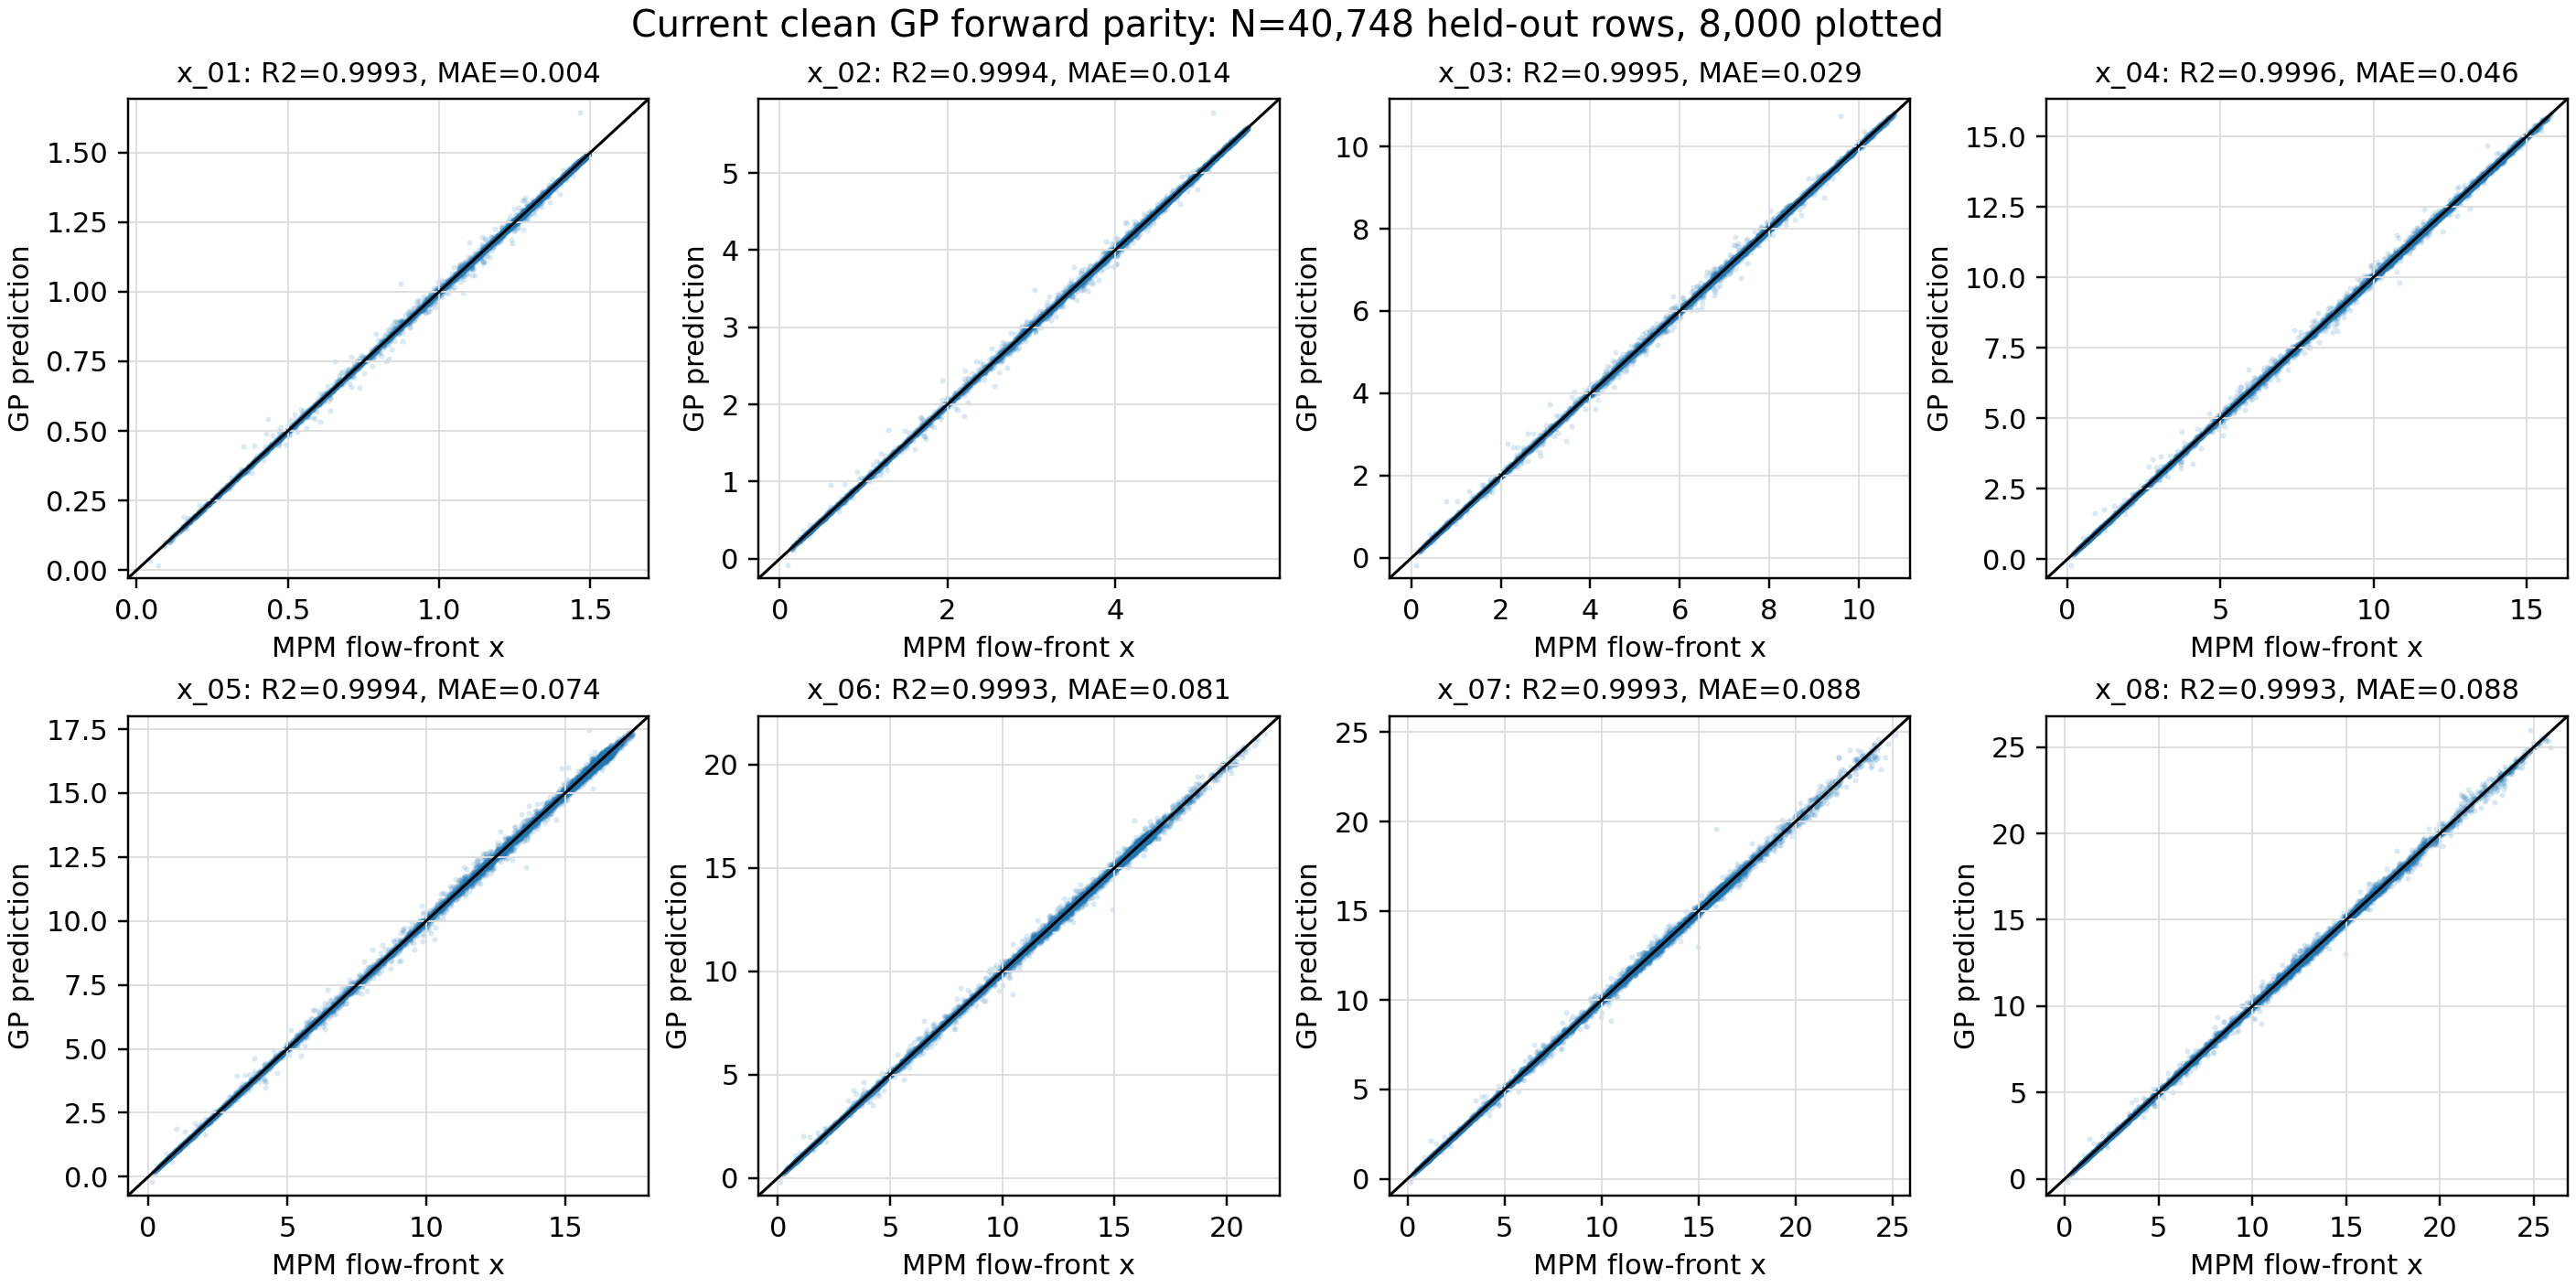
\includegraphics[width=\textwidth]{figs/true_vs_pred_current_gp.png}
    \caption{Surrogate parity on $N=40{,}748$ held-out
    quality-controlled MPM rows,
    one panel per flow-front frame $d=1\!\dots\!8$. Each row is
    forwarded by its assigned local GP expert; points are an
    $8{,}000$-row random subsample. Per-frame $R^2$ and MAE are
    computed over all $40{,}748$ rows. The plotted range spans more
    than two orders of magnitude in flow-front distance, and the
    remaining spread around the identity is quantified by the
    per-frame errors in Tab.~\ref{tab:fidelity}.}
    \Description{Eight scatter plots of surrogate-predicted flow-front
    displacement versus MPM ground truth across 40748 held-out
    samples; the cloud follows the identity trend across the full
    range for each of the eight flow-front frames.}
    \label{fig:parity}
\end{figure*}

\paragraph{Forward uncertainty and BAE.}
Because the inverse loop weights residuals by the forward uncertainty
(\S\ref{sec:inv-loss}), the default forward does not use
$\Sigma_{\mathrm{GP}}$ alone. Each expert stores validation residual
statistics, yielding a diagonal BAE term
$\Sigma_{\mathrm{BAE,expert}}$ that is added to the GP posterior
variance and observation noise. All $2{,}775$ experts store a BAE
variance entry; expert-local validation counts have min/median/max
$0/8/430$, with the $40$
validation-empty small-data experts shrunk toward the global residual
variance. For $x_{08}$, the global residual mean is $-0.00070$\,cm,
the residual standard deviation is $0.13782$\,cm, and the absolute
residual $p_{95}$ is $0.28195$\,cm. The reported inverse uses these
variance terms without an additional learned residual corrector.

\begin{table}[!htbp]
\centering
\footnotesize
\setlength{\tabcolsep}{4pt}
\caption{Forward uncertainty and BAE components used by the inverse.
Only variance terms enter the main GP-surrogate score.}
\label{tab:bae-diagnostics}
\begin{tabular}{@{}p{0.28\linewidth}p{0.28\linewidth}p{0.34\linewidth}@{}}
\toprule
Component & Main use & Evidence in this study \\
\midrule
GP posterior variance
  & included in $\Sigma_{\mathrm{forward}}$
  & exact local GP variance for each frame and expert \\
Expert BAE diagonal variance
  & included in $\Sigma_{\mathrm{forward}}$
  & BAE variance entries for $2{,}775/2{,}775$ experts; local validation count
    min/median/max $0/8/430$ \\
Observation noise
  & included in $\Sigma_{\mathrm{forward}}$
  & fixed noise floor shared across inverse runs \\
Global BAE for validation-empty experts
  & variance shrinkage
  & $40$ validation-empty small-data experts shrink toward global residual;
    $x_{08}$ residual std. $0.13782$\,cm, abs. $p_{95}=0.28195$\,cm \\
\bottomrule
\end{tabular}
\end{table}

\begin{figure}[!htbp]
    \centering
    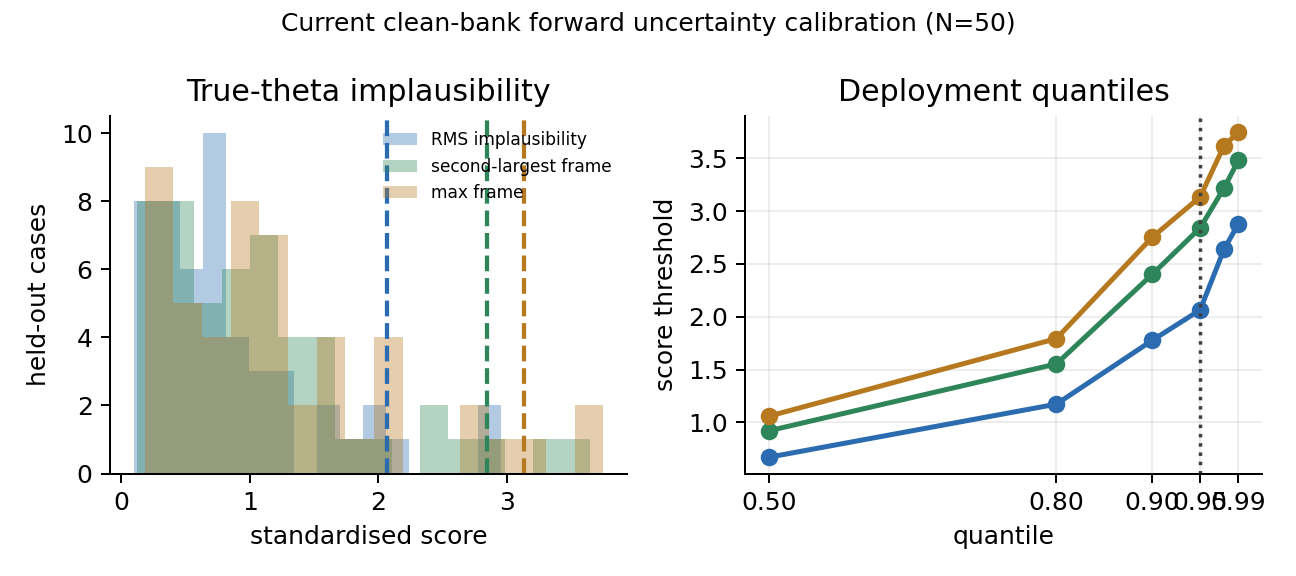
\includegraphics[width=\columnwidth]{figs/sigma_calibration.png}
    \caption{Forward uncertainty calibration for the local GP forward
    emulator trained on the quality-controlled fixed-density MPM corpus
    on $50$ held-out test rows. For each row,
    the true
    $\boldsymbol{\theta}$ is scored under the routed local GP,
    expert-level BAE variance, and observation-noise floor. The dashed
    lines and right panel report empirical score quantiles used as
    conservative plausibility gates; at $95\%$, the RMS,
    second-largest-frame, and max-frame implausibility thresholds are
    $2.06$, $2.84$, and $3.13$, respectively.}
    \Description{Two-panel forward uncertainty calibration plot. The
    left panel shows histograms of true-theta RMS, second-largest-frame,
    and max-frame implausibility scores over 50 held-out rows; the
    right panel shows the corresponding empirical quantile curves.}
    \label{fig:sigma-cal}
\end{figure}

Tab.~\ref{tab:fidelity} therefore establishes that the local GP bank
reproduces MPM forward outputs to sub-cm accuracy on held-out test
data. The BAE variance then carries the residual surrogate error into
the inverse objective, reducing overconfident use of the GP mean when
ranking candidates.


\subsection{Validation with Synthetic 3D Emulations}
\label{sec:mainresults}

Following the validation protocol
of~\citet{hamamichi2023nonnewtonian}, we first test the inverse on
synthetic dam-break observations whose ground-truth parameters are
known by construction. In the surrogate-inverse setting, a
top-$1$ point estimate is not the only relevant output: single-setup
dam-break observations can leave a ridge of plausible
Herschel--Bulkley parameters. We therefore report both point-estimate
accuracy and plausible-set quality. A valid inverse result may either
select the correct basin or retain it for subsequent setup
disambiguation. We run the full pipeline on synthetic materials drawn
from the calibrated parameter box of \S\ref{sec:data}, and report
the Hamamichi-normalised relative error
\begin{equation}
\label{eq:erel}
\begin{aligned}
E_{\mathrm{rel}}
&= \Bigg[
\biggl(\frac{\hat n-n^{\!\star}}{n_{\max}-n_{\min}}\biggr)^{\!2}
+
\biggl(\frac{\hat\eta-\eta^{\!\star}}{\eta_{\max}-\eta_{\min}}\biggr)^{\!2}
\\[-1mm]
&\qquad+
\biggl(\frac{\hat\sigma_Y-\sigma_Y^{\!\star}}
{\sigma_{Y,\max}-\sigma_{Y,\min}}\biggr)^{\!2}
\Bigg]^{1/2}.
\end{aligned}
\end{equation}
introduced by~\citet{hamamichi2023nonnewtonian}, with the parameter
box of \S\ref{sec:data} setting the normalisation. Following their
protocol, $E_{\mathrm{rel}}\le 0.1$ is a point-recovery threshold.
Because this range-normalised distance can understate errors in
log-spread variables, we use the log-parameter distance
$E_z$ from Eq.~\eqref{eq:Ez} for the synthetic plausible-set tables.
A candidate is counted as near truth when $E_z \le 0.25$, matching the
gate used by the validation scripts. The plausible-set diagnostics
then ask whether the set contains a near-truth candidate, how small
that set is, how many separate basins remain, and whether the
best-scored point lies in a false basin.

The predecessor evaluates synthetic materials with known parameters,
declares $E_{\mathrm{rel}}\le0.1$ as good enough, and applies the
setup-selection loop case by case.  Starting from one dam-break setup,
the inverse returns a current estimate; if the case is still ambiguous,
the Hessian-based proposer chooses the next setup intended to cut
across the local ridge.  The inverse is then rerun jointly on setups
$1/2$, then on setups $1/2/3$, and finally on setups $1/2/3/4$.
We keep this causal structure, but replacing MPM by a GP surrogate adds
a new question: whether the score selects the correct basin, or merely
retains it while ranking a surrogate-favoured false basin higher. The
tables below therefore separate plausible-set coverage, ranking
accuracy, retained-set size, and sequential shrinkage rather than
compressing them into a single point-estimate pass rate.

All synthetic panels in this section use the same clean GP forward,
BAE/error-aware objective, candidate generator, calibration gates, and
fixed evaluation configuration.

\paragraph{Sixty-four-case plausible-set stress test.}
We next evaluate the surrogate inverse on $64$ held-out synthetic
  cases. This panel uses a 512-candidate retrieval pool, the GP+BAE
  score, empirical calibration gates, and the same normalised parameter
distance for all setup counts. The evaluated set contains case
summaries and plausible representatives for every evaluated case.
Tab.~\ref{tab:retained-contract} summarises the main result. The
plausible set contains a near-truth representative in
$98.4$--$100.0\%$ of cases under the log-space $E_z$ criterion, while
the best-scored single candidate is close in only $6.3$--$14.1\%$ of
cases. To align this result with the predecessor's synthetic protocol,
Tab.~\ref{tab:erel-synthetic} also reports the same rank-$1$ and
best-retained candidates under the Hamamichi-normalised
$E_{\mathrm{rel}}$ criterion. Under that more permissive range-normalised
metric, rank-$1$ point recovery is $37.5$--$51.6\%$, and the retained
set contains an $E_{\mathrm{rel}}\le0.1$ candidate in all evaluated
cases. The method therefore supports a plausible-set inverse claim at
this stage, while the automatic selection of a unique
single-parameter triple remains metric-dependent and not yet reliable
under the stricter log-scale criterion.

\begin{table*}[!htbp]
\centering
\footnotesize
\setlength{\tabcolsep}{4pt}
\caption{$64$-case plausible-set stress test. ``Plausible close''
counts cases whose plausible set contains a near-truth representative
($E_z\le0.25$); ``selected close'' counts cases where the best-scored
single candidate is already near truth. ``Best $E_z$'' is the smallest
$E_z$ inside the plausible set and therefore measures candidate
coverage; it is not the same as automatic ranking accuracy. Plausible
fraction and basin count diagnose ambiguity, not automatic ranking
accuracy.}
\label{tab:retained-contract}
\begin{tabular}{@{}cccccccc@{}}
\toprule
Setups & Cases & Plausible close & Selected close
& Best plausible $E_z$ p50 & Best plausible $E_z$ p90 & Plausible fraction p50 & Basin p50 \\
\midrule
1 & $64$ & $98.4\%$ & $7.8\%$  & $0.099$ & $0.154$ & $0.574$ & $34.0$ \\
2 & $64$ & $100.0\%$ & $6.3\%$ & $0.084$ & $0.157$ & $0.559$ & $39.5$ \\
3 & $64$ & $98.4\%$ & $10.9\%$ & $0.079$ & $0.153$ & $0.359$ & $35.0$ \\
4 & $64$ & $98.4\%$ & $14.1\%$ & $0.078$ & $0.147$ & $0.273$ & $36.5$ \\
\bottomrule
\end{tabular}
\end{table*}

\begin{table*}[!htbp]
\centering
\footnotesize
\setlength{\tabcolsep}{4pt}
\caption{The same $64$-case synthetic panel evaluated with the
predecessor-style range-normalised parameter distance
$E_{\mathrm{rel}}$ from Eq.~\eqref{eq:erel}. ``Rank-1 pass'' uses the
best-scored single candidate and the Hamamichi threshold
$E_{\mathrm{rel}}\le0.1$; ``best retained'' reports the closest
candidate inside the retained plausible set. These numbers are reported
alongside Tab.~\ref{tab:retained-contract} because $E_{\mathrm{rel}}$
matches the predecessor's point-recovery protocol, whereas $E_z$
penalises order-of-magnitude mistakes in $\eta$ and $\sigma_Y$ more
strongly.}
\label{tab:erel-synthetic}
\begin{tabular}{@{}ccccccc@{}}
\toprule
Setups & Cases & Rank-1 pass & Rank-1 $E_{\mathrm{rel}}$ p50
& Rank-1 $E_{\mathrm{rel}}$ p90
& Best-retained pass & Best-retained $E_{\mathrm{rel}}$ p50 / p90 \\
\midrule
1 & $64$ & $37.5\%$ & $0.167$ & $0.443$ & $100.0\%$ & $0.008$ / $0.026$ \\
2 & $64$ & $42.2\%$ & $0.128$ & $0.530$ & $100.0\%$ & $0.006$ / $0.020$ \\
3 & $64$ & $51.6\%$ & $0.096$ & $0.528$ & $100.0\%$ & $0.005$ / $0.023$ \\
4 & $64$ & $50.0\%$ & $0.101$ & $0.508$ & $100.0\%$ & $0.004$ / $0.026$ \\
\bottomrule
\end{tabular}
\end{table*}

This separation between plausible-set recovery and selected-point recovery is the
central inverse diagnosis. The forward emulator is accurate at the
reported held-out MPM level, and the GP/BAE variance makes candidate
scoring explicitly error-aware, but this does not by itself solve
ranking: the objective can still prefer a surrogate-favoured false
basin inside a physically plausible ridge. The best plausible candidate
is close under both the predecessor-normalised and log-parameter
distances, but the median plausible basin count remains large, so the
pipeline should report ambiguity rather than collapse the posterior to a
single $\boldsymbol{\theta}$. This is the main limitation of the current
surrogate inverse and is reported directly rather than hidden by choosing
a different selector.

\paragraph{Causal four-setup audit.}
To mirror the predecessor's sequential protocol more directly, we also
run a $30$-case causal audit.  Setup~1 is fixed, the setup~1 inverse
produces a retained set, and the Hessian-orthogonal proposer selects
setup~2 from that current ambiguity. The joint setup~1/2 inverse then
selects setup~3, and the joint setup~1/2/3 inverse selects setup~4.
Tab.~\ref{tab:hessian-seq30} reports each accumulated setup set. The
retained fraction shrinks from $0.580$ after one setup to $0.258$
after four setups, matching the intended disambiguation direction.
However, near-truth retention also drops from $96.7\%$ to $90.0\%$,
and rank-1 recovery remains poor. Thus the GP surrogate currently
reproduces the \emph{workflow} of the multi-setup protocol, but its
validated claim is retained-set disambiguation rather than
predecessor-style automatic point recovery.

\begin{table}[!htbp]
\centering
\footnotesize
\setlength{\tabcolsep}{4pt}
\caption{Causal Hessian sequential audit on $30$ held-out synthetic
cases.  Each row uses the accumulated setups selected up to that stage.
``Retained close'' asks whether the plausible set still contains a
near-truth candidate; ``Rank-1 close'' asks whether the best-scored
candidate is near truth.}
\label{tab:hessian-seq30}
\begin{tabular}{@{}ccccc@{}}
\toprule
Setups & Retained close & Rank-1 close & Plausible fraction p50 & Basin p50 \\
\midrule
1 & $96.7\%$ & $3.3\%$ & $0.580$ & $25.5$ \\
2 & $100.0\%$ & $3.3\%$ & $0.457$ & $29.0$ \\
3 & $93.3\%$ & $3.3\%$ & $0.350$ & $25.5$ \\
4 & $90.0\%$ & $0.0\%$ & $0.258$ & $23.0$ \\
\bottomrule
\end{tabular}
\end{table}

\paragraph{Parameter-tail audit.}
Because $\eta$ and $\sigma_Y$ span several orders of magnitude, the
synthetic validation also records where cases fall in the logarithmic
parameter box.  This audit is necessary because range-normalized
errors can hide failures at the small- and large-value tails. In the
four-setup sequential audit, middle-$\eta$ cases retain a near-truth
candidate in $14/14$ cases, high-$\eta$ cases in $8/9$, and low-$\eta$
cases in $5/7$. For $\sigma_Y$, the high tail is sparse but
problematic: $2/3$ high-$\sigma_Y$ cases retain a near-truth candidate,
while all $5/5$ low-$\sigma_Y$ cases do. The two cases extreme in both
$\eta$ and $\sigma_Y$ retain the near-truth basin in only $1/2$ cases.
These tail diagnostics prevent the aggregate retained-close rate from
hiding failures at the edges of the rheological parameter box.

\paragraph{Flow-level replay.}
The retained-set tables evaluate whether a near-truth parameter remains
plausible, while dam-break replay error can remain small along parts of
the HB ridge. We therefore treat synthetic flow-curve overlays as a
supplementary diagnostic and keep the main synthetic evidence focused
on retained-set survival, rank, shrinkage, and tail behaviour.

\subsection{Validation with Real-World Experiments}
\label{sec:rheometer}

The real-fluid validation is restricted to the six Hamamichi
materials for which we have both dam-break captures and
parallel-plate rheometer sweeps: Chuno, Okonomiyaki sauce,
moisturising milk, lotion, Japanese pork-cutlet sauce, and sweet
bean paste.  This keeps the real comparison tied to independent
instrumental measurements rather than to another video inverse. In
the validation hierarchy used here this panel is diagnostic domain
validation: real observations include camera noise and MPM/HB model
discrepancy, so the success criterion is held-out prediction,
flow-curve agreement, and discrepancy size rather than synthetic
$E_{\mathrm{rel}}$.  For each material we evaluate one or two
dam-break setups with the same GP-surrogate inverse interface used in
the synthetic experiments. When the plausible set remains ambiguous,
the reported curve is read as one representative supported solution and
the ambiguity is part of the diagnostic. We then overlay the recovered
Herschel--Bulkley flow curve against the rheometer reference over the
shear-rate range probed by the dam-break replay.

This panel is an anchor rather than the final application regime of
the method. We use the six rheometer materials to measure how the
recovered \emph{flow curves} and replays compare with independent
rheometer fits over the shear-rate regime supported by the dam-break
observation, not to treat the rheometer fit as if it had zero model
discrepancy with the dam-break MPM model. The comparison is therefore
reported in three coupled spaces: the HB flow curve against the
parallel-plate reference, the eight-frame flow-front trajectory used
by the inverse, and binary/silhouette support in image space. The clean
Method does not use the rheometer sweep, replay mask error, or material
identity to choose a parameter. We therefore read this panel as a
post-hoc validation of the surrogate inverse output and as a diagnostic
of real/simulator mismatch, following validation practice that separates
model-use decisions from the independent data used to assess them
~\cite{bayarri2007framework,oberkampf2002verification,sargent2013verification}.

For completeness, we also keep the earlier real/simulator-gap branch as
a labelled diagnostic rather than as the main Method. In that branch, a
flow-curve-oriented diagnostic candidate has mean/worst
$E_{\mathrm{flow}}=0.100/0.137$ over the six material pairs, while an
image-replay diagnostic candidate has mean front and final-front replay
errors $0.306/0.341$\,cm. These two diagnostics are intentionally not
collapsed into a single material parameter: their disagreement estimates
the scale of the real/simulator gap and the ambiguity left by the
eight-front observation.

The same diagnostic branch includes several negative checks that prevent
it from being promoted to the clean Method. Under a strict
cross-application audit, only $2/6$ materials give the same compact
candidate across the video and flow-curve diagnostics, and another
$2/6$ are response-equivalent under the HB0.22 distance boundary. Chuno
and sweet bean paste remain split cases. With budgets
$0.22/0.30\,\mathrm{cm}/0.50\,\mathrm{cm}$ for flow-curve error, front
error, and final-front error, no split candidate is jointly feasible:
the nearest Chuno candidate has $0.316/0.415/0.774$, and the nearest
sweet bean paste candidate has $0.278/0.245/0.440$. Local real-gap
refocusing improves rheometer-flow residuals for those two materials to
$0.061$ and $0.093$, but the refocused candidates fail replay
validation. Interpolation between the flow-oriented and replay-oriented
endpoints also gives no clean repair. These audits remain
failure-analysis evidence and are not used to choose the clean inverse
output.

A rheometer flow curve and a dam-break video sample a material in
different regimes. The rheometer imposes controlled, approximately steady
shear rates, whereas the dam-break experiment produces a transient,
spatially heterogeneous free-surface flow. Agreement with a rheometer
flow curve therefore should not be interpreted uniformly over the entire
sweep; the relevant question is which shear-rate regimes are excited by
the real validation setup
~\citep{balmforth2007two,pashias1996fifty,ahmadi2022identification,muchiri2024identification}.

To audit this regime, we replay each measured real-material setup using
the HB fit obtained from the rheometer sweep as a reference material. We
then record the equivalent shear rate
$\dot\gamma_{\mathrm{eq}}=\sqrt{2D:D}$ for all fluid particles over the
eight observed frames. This diagnostic is computed from the
rheometer-reference material in the actual experimental geometries; it
is not computed from the inverse candidate parameters. The histograms in
Fig.~\ref{fig:gammadot-real} therefore characterize the shear-rate
support of the real validation videos themselves.

We interpret this support through the HB transition scale
$\dot\gamma^\star=(\sigma_Y/\eta)^{1/n}$ from
Eq.~\eqref{eq:gammastar}. Setup pairs that sample both the
yield-sensitive and viscous/power-law-dominated regimes can provide
complementary information about $\sigma_Y$ and $(\eta,n)$. In contrast,
two setups whose shear-rate distributions remain in the same regime
provide more redundant information and may leave a continuum of
near-equivalent HB parameters.

The dam-break p5--p95 supports in Tab.~\ref{tab:gammadot-real} all lie
inside the measured rheometer interval $0.1$--$1000\,\mathrm{s}^{-1}$,
but they occupy only a subset of that interval. Thus flow-curve
agreement should be read most strongly over the overlap between the
rheometer sweep and the dam-break shear-rate support. Agreement outside
that support is a post-hoc HB extrapolation diagnostic rather than
direct video-supported validation. The setup pairs in this audit are
the measured real-material validation setups used by the inverse, not
pairs selected to maximise $\dot\gamma$ coverage; a separate
candidate-setup sweep would be required to claim maximal shear-rate
coverage.

Tab.~\ref{tab:rheo-recovery} lists a two-setup post-hoc flow-curve
diagnostic from the local GP surrogate trained on the quality-controlled
fixed-density MPM corpus.
Fig.~\ref{fig:flow-real} shows the regenerated flow-curve overlays,
and Fig.~\ref{fig:real-snapdiff}
shows the corresponding binary-mask replay check in the predecessor-style
snap-difference layout: real foregrounds, MPM foregrounds, and
amplified pairwise differences are shown across the observed frames for
a representative Chuno setup. The shear-rate support audit in
Fig.~\ref{fig:gammadot-real} determines how strongly these replay and
flow-curve diagnostics should be interpreted as evidence about the
rheometer curve: agreement is most direct where the real dam-break
setups actually excite the relevant shear-rate regime, and agreement
outside that support is an HB-model extrapolation check.

The numerical $\hat{\boldsymbol{\theta}}$ values in
Tab.~\ref{tab:rheo-recovery} are diagnostic candidates used to draw the
flow-curve validation panel, not a claim that every real material has a
unique recovered parameter triple. The clean Method reports a unique
theta only when the retained set is compact by the simulator-calibrated
criteria of \S\ref{sec:inv-ranking}; otherwise the retained set remains
the output and the real panels are interpreted as validation diagnostics.

\begin{table}[!htbp]
\centering
\footnotesize
\setlength{\tabcolsep}{4pt}
\caption{Real-material two-setup flow-curve diagnostic. $E_{\mathrm{flow}}$ is the log-stress RMS
distance to the rheometer sweep over
$\dot\gamma\in[1,398]\,\mathrm{s}^{-1}$; visual agreement is shown in
Fig.~\ref{fig:flow-real}. These candidates are not used to define the
clean inverse objective or thresholds; the flow error is a post-hoc
validation metric.}
\label{tab:rheo-recovery}
\begin{tabular}{@{}lcccccc@{}}
\toprule
Material  & $(W_1,H_1)$ & $(W_2,H_2)$
          & $\hat n$ & $\hat\eta$ & $\hat\sigma_Y$ & $E_{\mathrm{flow}}$ \\
\midrule
Chuno              & $(2.5, 2.7)$ & $(4.0, 2.0)$
                    & $0.75$ & $6.0$  & $21.9$ & $0.074$ \\
Okonomiyaki        & $(2.2, 2.5)$ & $(7.0, 7.0)$
                    & $0.34$ & $144.1$  & $3.0$ & $0.046$ \\
Moisturising milk  & $(4.5, 3.5)$ & $(4.5, 2.0)$
                    & $0.68$ & $18.2$  & $115.1$ & $0.135$ \\
Lotion             & $(6.1, 2.8)$ & $(7.0, 6.5)$
                    & $0.94$ & $10.3$ & $172.8$ & $0.122$ \\
Pork-cutlet sauce  & $(6.5, 2.1)$ & $(7.0, 7.0)$
                    & $0.47$ & $32.5$  & $41.3$  & $0.084$ \\
Sweet bean paste   & $(4.8, 4.1)$ & $(2.5, 2.5)$
                    & $0.49$ & $225.1$ & $55.1$ & $0.137$ \\
\bottomrule
\end{tabular}
\end{table}

\begin{table}[!htbp]
\centering
\footnotesize
\setlength{\tabcolsep}{4pt}
\caption{Dam-break shear-rate support under the rheometer-reference HB
material model. For each real material, the two measured validation
setups are replayed using the HB fit to the rheometer sweep, and
$\dot\gamma_{\mathrm{eq}}=\sqrt{2D:D}$ is pooled over all fluid
particles and observed frames. The p5, p50, and p95 values describe the
shear-rate regimes actually probed by the real dam-break videos. These
values bound the interpretation of the flow-curve overlays; they do not
imply maximal setup coverage or validation of the entire rheometer
sweep.}
\label{tab:gammadot-real}
\begin{tabular}{@{}lccc@{}}
\toprule
Material & $\dot\gamma_{p5}$ & $\dot\gamma_{p50}$ &
$\dot\gamma_{p95}$ \\
\midrule
Chuno              & $1.70$ & $11.54$ & $35.99$ \\
Okonomiyaki        & $0.30$ & $4.88$  & $35.63$ \\
Moisturising milk  & $0.18$ & $4.58$  & $26.34$ \\
Lotion             & $0.17$ & $5.16$  & $33.98$ \\
Pork-cutlet sauce  & $0.36$ & $7.88$  & $63.89$ \\
Sweet bean paste   & $0.11$ & $1.95$  & $6.99$ \\
\bottomrule
\end{tabular}
\end{table}

\begin{figure*}[!htbp]
    \centering
    \begin{tabular}{ccc}
        \figureorplaceholder[2.45cm]{0.30\textwidth}{figs/real_world/real6_chuno_gamma_dot_coverage.png}{(a) Chuno shear-rate histogram.} &
        \figureorplaceholder[2.45cm]{0.30\textwidth}{figs/real_world/real6_okonomiyaki_gamma_dot_coverage.png}{(b) Okonomiyaki shear-rate histogram.} &
        \figureorplaceholder[2.45cm]{0.30\textwidth}{figs/real_world/real6_moisturising_milk_gamma_dot_coverage.png}{(c) Moisturising milk shear-rate histogram.}\\
        \figureorplaceholder[2.45cm]{0.30\textwidth}{figs/real_world/real6_lotion_gamma_dot_coverage.png}{(d) Lotion shear-rate histogram.} &
        \figureorplaceholder[2.45cm]{0.30\textwidth}{figs/real_world/real6_tonkatsu_gamma_dot_coverage.png}{(e) Japanese pork-cutlet sauce shear-rate histogram.} &
        \figureorplaceholder[2.45cm]{0.30\textwidth}{figs/real_world/real6_sweetbean_gamma_dot_coverage.png}{(f) Sweet bean paste shear-rate histogram.}
    \end{tabular}
    \caption{Shear-rate coverage of the real validation setups.
    Histograms show $\log_{10}\dot\gamma_{\mathrm{eq}}$ for the
    rheometer-reference material replayed in the two setup geometries
    used by the real experiments. Red denotes setup~1 and blue denotes
    setup~2. The gray interval marks the rheometer-measured shear-rate
    range, dashed vertical lines mark the HB-fit interval used for
    flow-curve comparison, and the dotted vertical line marks the HB
    transition scale $\dot\gamma^\star$. These plots audit the
    shear-rate support of the real videos; they are not histograms of
    the inverse candidate parameters.}
    \Description{Six log-shear-rate histograms showing that the
    dam-break support for setup 1 and setup 2 lies inside the
    rheometer-measured shear-rate interval for the real-material
    validation panel, with the HB transition scale marked in each
    panel.}
    \label{fig:gammadot-real}
\end{figure*}

The material-wise patterns in Fig.~\ref{fig:gammadot-real} explain why
the measured setup pairs are not equally informative. Okonomiyaki,
lotion, and pork-cutlet sauce show clear setup complementarity: one
setup samples lower or transition shear rates, while the other shifts
the response toward higher, more viscous-dominated rates. These cases
are better positioned to reduce the coupling between yield-stress and
viscous/power-law parameters. Moisturising milk also spans the
transition regime, but its selected representative does not
substantially improve the flow-curve diagnostic over the raw current
candidate, showing that regime coverage is informative but not
sufficient to guarantee a better point estimate.

Chuno and sweet bean paste illustrate the limitations of the available
real setups. For Chuno, both setups mainly probe shear rates above the
transition scale, so the videos provide weaker independent information
about the yield-dominated regime. For sweet bean paste, both setups
remain concentrated in the low-to-transition range, with p95 support
only about $7\,\mathrm{s}^{-1}$. Consequently, high-shear agreement in
the sweet-bean-paste flow-curve overlay should be treated as model
extrapolation rather than direct evidence from the dam-break videos.

\begin{figure*}[!htbp]
    \centering
    % Row 1: 3 panels
    \begin{minipage}[t]{0.32\textwidth}
        \centering
        \figureorplaceholder[2.45cm]{\linewidth}{figs/real_world/real6_chuno_flowcurve_single_vs_joint.png}{(a) Chuno: rheometer, raw GP-score minimizer, and diagnostic candidate.}\\
        {\footnotesize (a) Chuno (Japanese thickened sauce)}
    \end{minipage}\hfill
    \begin{minipage}[t]{0.32\textwidth}
        \centering
        \figureorplaceholder[2.45cm]{\linewidth}{figs/real_world/real6_okonomiyaki_flowcurve_single_vs_joint.png}{(b) Okonomiyaki: rheometer, raw GP-score minimizer, and diagnostic candidate.}\\
        {\footnotesize (b) Okonomiyaki (cabbage pancake sauce)}
    \end{minipage}\hfill
    \begin{minipage}[t]{0.32\textwidth}
        \centering
        \figureorplaceholder[2.45cm]{\linewidth}{figs/real_world/real6_moisturising_milk_flowcurve_single_vs_joint.png}{(c) Moisturising milk: rheometer, raw GP-score minimizer, and diagnostic candidate.}\\
        {\footnotesize (c) Moisturising milk}
    \end{minipage}\\[4pt]
    % Row 2: 3 panels
    \begin{minipage}[t]{0.32\textwidth}
        \centering
        \figureorplaceholder[2.45cm]{\linewidth}{figs/real_world/real6_lotion_flowcurve_single_vs_joint.png}{(d) Lotion: rheometer, raw GP-score minimizer, and diagnostic candidate.}\\
        {\footnotesize (d) Lotion}
    \end{minipage}\hfill
    \begin{minipage}[t]{0.32\textwidth}
        \centering
        \figureorplaceholder[2.45cm]{\linewidth}{figs/real_world/real6_tonkatsu_flowcurve_single_vs_joint.png}{(e) Japanese pork-cutlet sauce: rheometer, raw GP-score minimizer, and diagnostic candidate.}\\
        {\footnotesize (e) Japanese pork-cutlet sauce}
    \end{minipage}\hfill
    \begin{minipage}[t]{0.32\textwidth}
        \centering
        \figureorplaceholder[2.45cm]{\linewidth}{figs/real_world/real6_sweetbean_flowcurve_single_vs_joint.png}{(f) Sweet bean paste: rheometer, raw GP-score minimizer, and diagnostic candidate.}\\
        {\footnotesize (f) Sweet bean paste}
    \end{minipage}
    \caption{Herschel--Bulkley flow curves recovered by the local GP
    surrogate on the six rheometer-reference materials, following the
    visual style of Fig.~13 in~\citet{hamamichi2023nonnewtonian}. Gray
    points are the measured parallel-plate sweep, black is the HB fit
    to that sweep, blue is the raw joint GP-score minimizer, and green
    is the post-hoc diagnostic candidate listed in
    Tab.~\ref{tab:rheo-recovery}. The green curves are validation
    diagnostics, not selectors used by the clean Method. The panel is
    interpreted together with the shear-rate support in
    Tab.~\ref{tab:gammadot-real} and Fig.~\ref{fig:gammadot-real}:
    agreement within the dam-break p5--p95 support is directly
    video-supported, whereas agreement outside that support is a
    post-hoc HB extrapolation diagnostic.}
    \Description{Two-by-three grid of log-log flow-curve overlays.
    Each panel shows a rotational-rheometer sweep, its HB fit, the
    raw joint GP-score minimizer, and a diagnostic candidate for
    one Hamamichi reference material.}
    \label{fig:flow-real}
\end{figure*}

\begin{figure*}[!htbp]
    \centering
    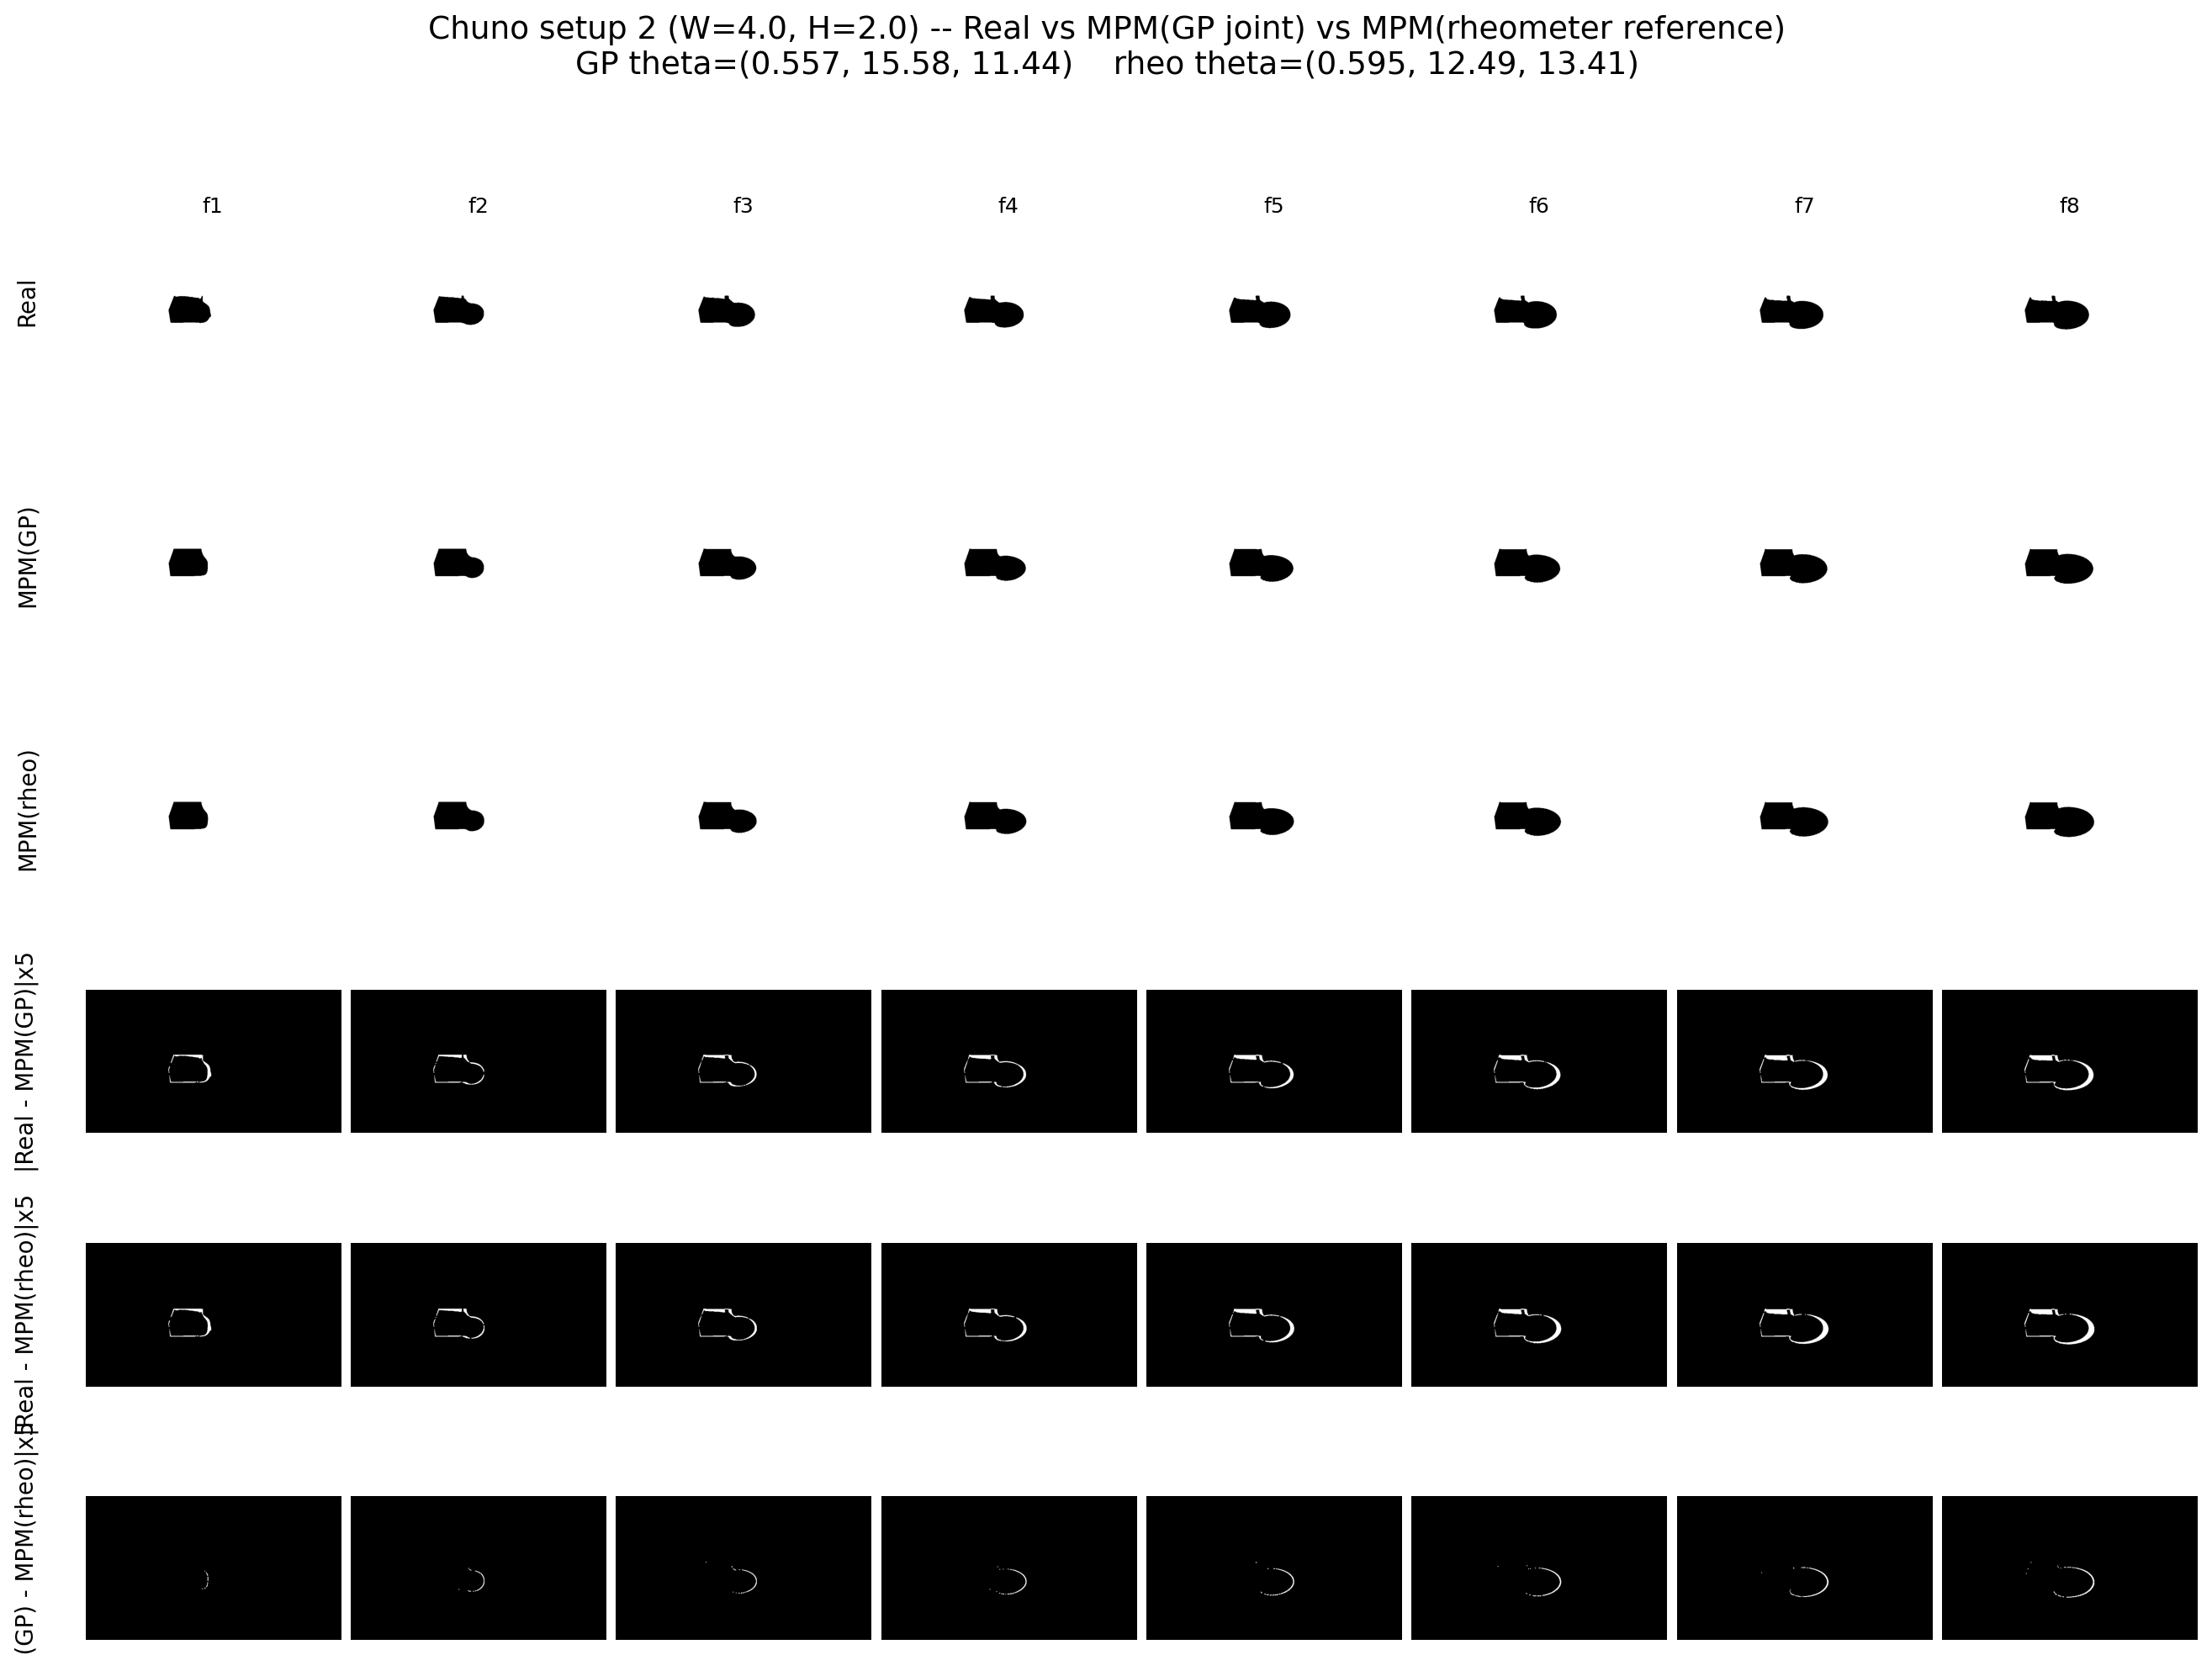
\includegraphics[width=0.88\textwidth]{figs/real_world/snapdiff_chuno_joint_current_gp.png}
    \caption{Binary snap-difference replay check in the
    predecessor-style layout, regenerated with the reported GP inverse result.
    The example shows the Chuno second setup under the same two-setup
    GP estimate used by the Chuno joint flow curve in
    Fig.~\ref{fig:flow-real}. The first rows show the segmented real
    frames, the MPM replay at the GP estimate, and the MPM replay at
    the rheometer-reference HB fit after conversion to the simulator
    parameter convention used for the simple-shear flow-curve
    calibration; the lower rows show amplified XOR foreground
    differences as white pixels on a black background. Together with
    the Chuno shear-rate support in Fig.~\ref{fig:gammadot-real}, this
    replay check is a visual diagnostic for sim--real discrepancy and
    GP-vs-rheometer replay behaviour, not a validation of the entire
    rheometer flow curve outside the shear-rate regimes excited by the
    videos.}
    \Description{Eight-frame binary-mask replay panel for the Chuno
    second setup, with observed masks, reported two-setup GP-estimate
    replay masks, rheometer-reference replay masks, and amplified
    black-background white-difference rows.}
    \label{fig:real-snapdiff}
\end{figure*}

Agreement at the parameter-triple level is not the only relevant bar
for video rheometry: the dam-break observation can lie on the
$(\eta,\sigma_Y)$-ridge of \S\ref{sec:inv-sy}, so multiple triples
may predict similar free-surface motion over the observed
shear-rate window. We therefore keep the six-material flow-curve panel
as the required diagnostic format instead of reducing it to a single
success count. Good overlays show where the video inverse agrees with
the parallel-plate reference; poor overlays identify materials or
geometries where the real--sim gap or the remaining
Herschel--Bulkley ridge dominates. The flow-curve overlays are
shown in Fig.~\ref{fig:flow-real}. The snap-difference panel in
Fig.~\ref{fig:real-snapdiff} adds a frame-level binary-mask check of
the same replay discrepancy for the representative Chuno case, while
the aggregate silhouette packet remains a numerical audit over all
twelve material/setup cases. The diagnostic flow-curve branch gives mean/worst
$E_{\mathrm{flow}}=0.100/0.137$, while the image-space replay branch
gives mean front/$x_8$ replay errors $0.306/0.341$\,cm. The contracted
twelve-case silhouette replay audit gives mean case-level IoU $0.886$
and minimum frame-level IoU $0.747$. These numbers are validation
diagnostics: they show how different post-hoc candidates expose
different parts of the real/simulator gap, and they are not fed back
into the clean inverse objective, thresholds, retained-set rule, or setup
policy. A separate bounded single-output sensitivity keeps one
diagnostic candidate for $5/6$ materials, with mean front/$x_8$ replay
errors $0.356/0.445$\,cm. The excluded $1/6$ material is sweet bean
paste; it stays in the same response basin under the budget but is not a
strict unique-theta case. A shared-nuisance diagnostic reduces the worst
flow residual to $0.223$ but has larger replay residuals
($0.688/0.875$\,cm). Thus this section establishes real-material
validation behavior and the approximate discrepancy scale; it does not
treat the rheometer fit as synthetic ground truth or promote a
replay-only diagnostic to the material-parameter selector.
Per-parameter uncertainty along
the ridge should be reported by plausible-set diameter, setup-wise
consistency, and optional local curvature diagnostics
(\S\ref{sec:inv-ranking}) rather than hidden by a hand-chosen prior.

\subsection{Application to Same-Session Freshness Checks}
\label{sec:freshness}

The predecessor's sequential two-setup protocol chooses setup~2 after
the setup~1 inverse returns. With simulation-in-the-loop optimisation,
this can create an hours-scale computational gap between captures. For
self-prepared or ageing materials, such a gap can mix observations from
different material states. The practical role of a seconds-scale
surrogate inverse is therefore not only lower runtime, but also the
ability to evaluate multiple setups while the material is still in the
same short-time state.

We test this consequence as a \emph{Freshness held-out setup diagnostic}.
For each short-time material group, three setups are captured in one
session; two short-time dam-break captures are used for inverse
estimation with the same clean surrogate interface, and the unused third capture from the same
session is held out for flow-front and binary-mask replay.
Unlike the rheometer panel in \S\ref{sec:rheometer}, these materials do
not provide independent flow-curve ground truth. The validation target
is therefore same-session predictive consistency: a parameter inferred
from two setups should replay the third setup's flow front and
segmented foreground reasonably well. This is not a fitted kinetic
ageing model.

\begin{table}[!htbp]
\centering
\footnotesize
\setlength{\tabcolsep}{4pt}
\caption{Freshness held-out setup check. Each case uses two
short-time setups for inverse and evaluates the unused third setup from
the same capture session. Flow-front errors are reported in
centimetres; binary-mask metrics compare the held-out segmented frame
to the predicted support mask.}
\label{tab:fresh-holdout}
\begin{tabular}{@{}lccccc@{}}
\toprule
Metric & cases & frames & mean & median & worst \\
\midrule
$x_{08}$ abs. error & $6$ & -- & $0.548$ & $0.268$ & $2.139$ \\
Median front abs. error & $6$ & -- & $0.297$ & $0.233$ & $0.712$ \\
Case-mean mask IoU & $6$ & $48$ & $0.902$ & $0.921$ & $0.803$ \\
Image XOR fraction & $6$ & $48$ & $0.0052$ & $0.0034$ & $0.0158$ \\
\bottomrule
\end{tabular}
\end{table}

The evaluated freshness set contains six material groups, each with a
held-out third setup. The held-out validation packet has mean
median-front error $0.297$\,cm, mean $x_{08}$ error $0.548$\,cm, and
mask IoU/XOR $0.902/0.0052$. These values are reported only after
inference and are not used to tune the inverse score, choose thresholds,
or choose a representative. EggFoam is the largest residual case, with
case-mean IoU $0.803$, foreground-error fraction $0.0158$, median front
error $0.712$\,cm, and $x_{08}$ error $2.139$\,cm. We therefore read
the result as a useful same-session predictive check with visible
failure cases, not as a universal freshness parameter estimator.

\begin{figure*}[!htbp]
    \centering
    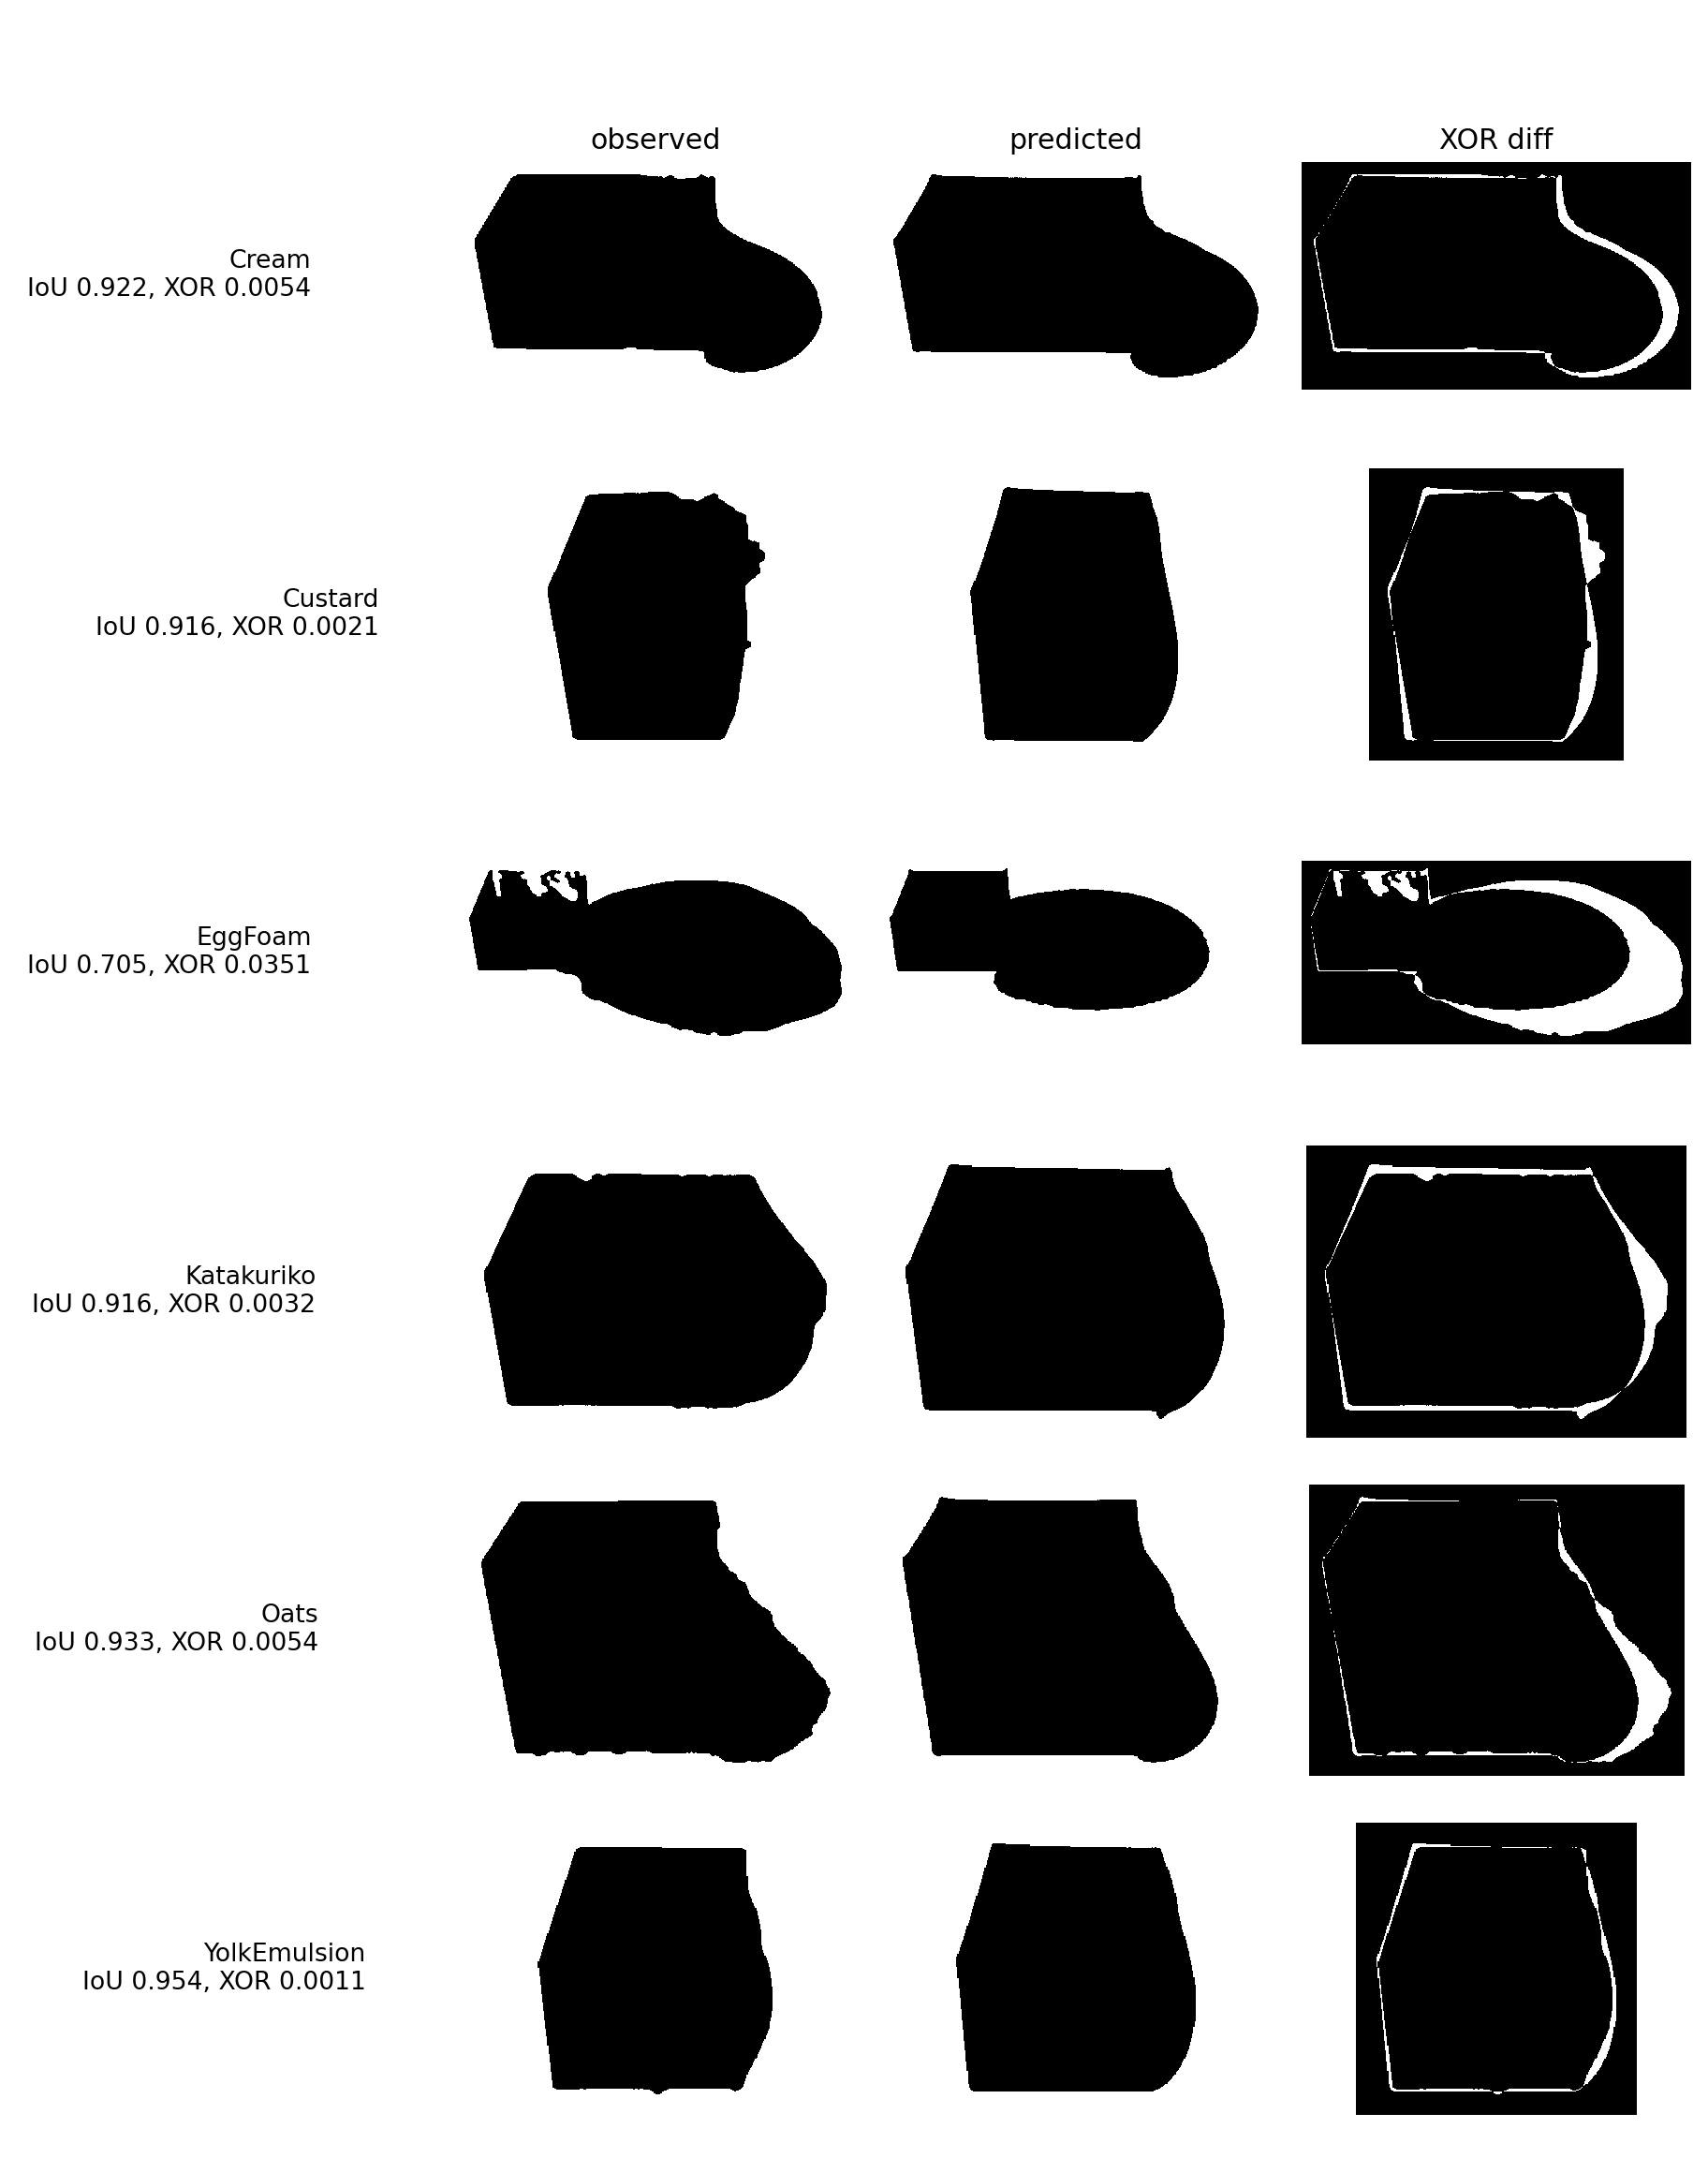
\includegraphics[width=0.72\textwidth]{figs/real_world/freshness_holdout_binary_diff_panel.png}
\caption{Held-out binary-mask freshness check on six
short-time material cases. Each row uses two setups for inverse and
visualises the unused held-out setup at frame~8. Columns show the
observed segmented foreground, the predicted foreground support,
and the XOR difference; row labels report the frame~8 IoU and XOR
fraction, while Tab.~\ref{tab:fresh-holdout} aggregates all replayed
frames. All six cases in
Tab.~\ref{tab:fresh-holdout} are included in this visual panel.}
    \Description{Six-row binary-mask comparison panel for the
    freshness held-out setup experiment, with observed masks,
    predicted masks, and XOR differences.}
    \label{fig:fresh-binary}
\end{figure*}

\paragraph{Claim boundary.}
This experiment shows that a two-setup estimate can be checked against
a third same-session setup. It does not estimate a material-ageing law;
that would require repeated time-indexed inverses and a separate
identifiability study for the chosen kinetic model. The validated claim
is narrower: seconds-scale inverse makes same-session held-out setup
validation practical.

\subsection{Compute-Stage Time Budget}
\label{sec:timebudget}

We time the automated inverse compute stage replaced by the GP surrogate.
The timing excludes preparation, capture, segmentation, and camera
calibration.
In the measured speed run, GP inverse primary scoring required
$1393.6$\,s for $64$ cases evaluated up to $6$ setups, or
$3.63$\,s per case/setup in the unoptimised Python implementation.
A single surrogate candidate/setup evaluation took $7.09$\,ms,
which is $190$--$618\times$ faster than the measured one-shot MPM
replay references used in the same timing study. Tab.~\ref{tab:time-budget}
reports the compute-stage breakdown. The multi-setup entries are the
measured per-case/setup average scaled by the number of accumulated
setups, not a separately optimised stopwatch implementation for each
row; operator-dependent manual timings are not used as a headline
validated result, and our entries are from the current GP-surrogate
speed artifact.

\begin{table}[!htbp]
\centering
\small
\caption{Validated compute-stage time budget after observations are
available. The predecessor inverse entries are the reported
simulation-in-the-loop runtimes from~\citet{hamamichi2023nonnewtonian};
our entries are measured from the reported GP-surrogate implementation.}
\label{tab:time-budget}
\begin{tabular}{@{}lccc@{}}
\toprule
Compute query & Predecessor & GP surrogate & Gain \\
\midrule
Single-setup inverse & $\sim 8$\,h & $3.6$\,s & $\sim8.0\times10^{3}$ \\
Two-setup inverse & $\sim 16$\,h & $7.3$\,s & $\sim7.9\times10^{3}$ \\
Four-setup inverse & $\sim 32$\,h & $14.5$\,s & $\sim7.9\times10^{3}$ \\
Six-setup inverse & $\sim 48$\,h & $21.8$\,s & $\sim7.9\times10^{3}$ \\
Single surrogate eval & $1.35$--$4.38$\,s & $0.0071$\,s & $190$--$618\times$ \\
\bottomrule
\end{tabular}
\end{table}

Thus the validated replacement of the simulation-in-the-loop inverse is
seconds-scale rather than hours-scale once the observation vector is
available. The practical effect is not only lower latency, but access to
held-out repeated-capture checks and multi-setup diagnostics inside a
single user session.
\section{Discussion and Conclusion}
\label{sec:discussion}

We presented a surrogate-accelerated framework for non-Newtonian
video rheometry that replaces MPM calls inside the inverse loop with a
local GP forward emulator and an error-aware inverse objective.
The forward model maps
$(n,\eta,\sigma_Y,W,H)$ to the eight-frame dam-break trajectory
$(x_{01},\ldots,x_{08})$ using a $2{,}775$-expert exact-GP bank
trained on $407{,}480$ cleaned MPM rows with fixed density $\rho=1.0$. Its uncertainty model
combines GP posterior variance, local BAE variance, and observation
noise, so the inverse does not treat the surrogate mean as exact. The
inverse then returns either a point estimate or an ambiguous plausible
set, and multi-setup experiments evaluate whether additional
observations shrink the plausible set while preserving a near-truth
basin. The observation pipeline also includes marker-based pose
initialisation and silhouette-edge refinement to place real captures in
the same geometric frame as the surrogate input, but the main validated
contribution here is the surrogate inverse and its error-aware
reporting.
\citet{hamamichi2023nonnewtonian} mitigates the same ridge with
Hessian-based similarity analysis, a Poiseuille-flow proxy, active
setup selection, and iterative multi-setup CMA-ES; our path
uses the GP surrogate to make such disambiguation tests cheap enough
to run as routine plausible-set validation rather than as rare
simulation-in-the-loop studies.

The validation results clarify both what the surrogate solves and what
it does not solve. The forward emulator is accurate enough for fast
candidate evaluation: on $40{,}748$ held-out MPM rows it achieves
overall MAE $0.05296$\,cm, RMSE $0.10605$\,cm, and
$R^2=0.9996376$, with final-frame $x_{08}$ MAE $0.08790$\,cm and
$x_{08}$ absolute-error p95 $0.28993$\,cm. The BAE audit places the
remaining final-frame residual scale at standard deviation
$0.13782$\,cm and p95 $0.28195$\,cm. These numbers support replacing
MPM by the GP bank inside the inverse score, provided that the residual
variance is carried into the likelihood. They do not imply that the
lowest-score inverse candidate is automatically correct.

The synthetic inverse results expose that distinction. In the
$64$-case stress test, the plausible set contains a near-truth candidate
in $98.4$--$100.0\%$ of cases from one to four setups, and the median
best-plausible $E_z$ improves from $0.099$ to $0.078$. Thus candidate
coverage is strong. Under the stricter log-parameter criterion, however,
the best-scored candidate is near truth in only $7.8\%$, $6.3\%$,
$10.9\%$, and $14.1\%$ of the one-, two-, three-, and four-setup cases.
Under the predecessor's range-normalised $E_{\mathrm{rel}}\le0.1$
criterion, the same rank-$1$ candidates pass in $37.5\%$, $42.2\%$,
$51.6\%$, and $50.0\%$ of cases, while the best retained candidate
passes in $100.0\%$ of cases for every setup count. The causal
$30$-case audit shows the same
pattern in the predecessor-style sequential protocol: the median
plausible fraction shrinks from $0.580$ after one setup to $0.258$
after four setups, but retained-close also drops from $96.7\%$ to
$90.0\%$ and rank-1 close remains $0$--$3.3\%$. Therefore the GP
surrogate reproduces the intended disambiguation workflow and shrinks
the candidate set, but the current score is still unreliable as an
automatic selector. The paper's inverse claim is accordingly
retained-set recovery and ambiguity reduction, not unique parameter
recovery.

The tail audit explains why this distinction matters. Middle-$\eta$
cases retain a near-truth candidate in $14/14$ cases, while low-$\eta$
and high-$\eta$ cases retain it in $5/7$ and $8/9$ cases; high
$\sigma_Y$ is sparser but weaker at $2/3$, and the two cases extreme in
both $\eta$ and $\sigma_Y$ retain the near-truth basin in only $1/2$
cases. These failures would be hidden by reporting only aggregate
forward $R^2$ or a single mean inverse error. They instead indicate
where additional MPM data, less aggressive plausibility gates, or
stronger setup evidence would be needed.

The real-material and freshness panels are interpreted as diagnostic
domain validations rather than synthetic-truth tests. For the six
rheometer-reference materials, one post-hoc flow-curve diagnostic gives
mean/worst $E_{\mathrm{flow}}=0.100/0.137$, while an image-space replay
diagnostic gives mean front/$x_8$ replay errors of $0.306/0.341$\,cm.
The contracted silhouette replay packet covers the twelve
material/setup cases and gives mean case-level IoU $0.886$ with minimum
frame-level IoU $0.747$. These summaries are not merged into one
universal material theta because their objectives expose different parts
of the real/simulator gap. Additional diagnostic audits show that the
split is not only a discrete-search artifact: local continuous refocus
can repair the rheometer-flow residuals for Chuno and sweet bean paste
($0.061$ and $0.093$ log-RMS), but the refocused parameters fail replay
validation; simple interpolation between the flow-oriented and
image-oriented endpoints also yields no clean joint repair. These
numbers include camera, segmentation, and real/simulator discrepancy, so
they are not synthetic parameter errors and are not used to tune the
clean inverse method. The gamma-dot audit shows that the measured
validation setups excite p5--p95 shear-rate supports inside the
$0.1$--$1000\,\mathrm{s}^{-1}$ rheometer interval, but only the overlap
with those dam-break supports is directly video-supported; agreement
outside that support is an HB extrapolation diagnostic. The
freshness panel shows that a two-setup estimate can replay a third
same-session setup with mean median-front error $0.297$\,cm, mean
$x_{08}$ error $0.548$\,cm, mean mask IoU $0.902$, and image XOR
fraction $0.0052$. EggFoam and YolkEmulsion are not counted as
application-level unique recoveries: EggFoam lacks enough complete
held-out replay evidence, while YolkEmulsion remains a
setup-generalization conflict. This supports a
repeated-capture protocol enabled by speed, not a kinetic ageing model
or a guarantee of unique recovery on every real material.

The main practical gain is amortisation. The expensive MPM corpus is
paid for once, while inverse queries, multi-setup ambiguity checks,
real-material replay diagnostics, and freshness hold-out tests run at
seconds scale on the trained surrogate: $3.6$\,s for one setup,
$14.5$\,s for four setups, and $21.8$\,s for six setups under the
reported implementation. The surrogate is therefore an accelerator for
a physics-grounded inverse, not a replacement for the physical model.


\section{Limitations and Future Work}
\label{sec:limitations}

There are several limitations in our work. First, the present inverse
does not guarantee that the lowest-score candidate is the true material
parameter. The GP bank is accurate on held-out MPM data, and the
retained sets usually contain a near-truth candidate in the synthetic
tests, but the rank-$1$ candidate is still unreliable. Thus the current
output should be read as an ambiguity-aware estimate: the method can
report plausible basins and test whether additional setups reduce them,
but it is not yet a fully automatic unique-parameter estimator. Future
work should improve this selector by validating it against held-out MPM
replays, relaxing overly aggressive plausibility gates, and calibrating
scores so that near-truth candidates are ranked ahead of false basins
that happen to fit the surrogate. For real materials, the negative
continuous-refocus and interpolation audits suggest that the remaining
split cases are not solved by a simple local score repair. They require
either richer observations, stronger setup evidence, or an explicit
real--simulation discrepancy model that is itself validated by replay.

Second, the range of setups and material parameters implicitly defines
the range where the estimate is reliable. The surrogate has been
validated for $W,H\in[2,7]$\,cm, fixed density $\rho=1.0$, and the
sampled Herschel--Bulkley parameter box. The synthetic tail audit shows
weaker retention near the extremes of $\eta$ and $\sigma_Y$, and the
real-material gamma-dot audit only checks the measured validation
setups rather than all feasible setups. It would be useful to
quantitatively investigate this shear-rate and parameter-space
coverage, and to add targeted MPM samples in the low-/high-$\eta$ and
high-$\sigma_Y$ regions where the retained-set test fails most often.

Third, the simulator and the real experiment are not identical. Thin
materials that spread very quickly may require surface tension and more
accurate gate-opening dynamics, while materials that barely flow may
not provide enough motion to identify all three HB parameters. The
real-material panel also includes camera calibration, segmentation,
wall/contact effects, and real--sim mismatch. The current MPM model
does not include surface tension, thixotropy, elastic overshoot,
viscoelastic memory, evaporation, or time-dependent ageing. The
freshness experiment should therefore be read as same-session
held-out setup validation enabled by seconds-scale inverse, not as a
fitted kinetic material model.

For future work, it would be beneficial to build a more complete
measurement device and application workflow. Automating the setting of
the dam-break dimensions, the opening of the front panel, camera
calibration, segmentation, setup proposal, inverse inference,
uncertainty reporting, held-out replay validation, and flow-curve
export would reduce the manual workload and make the method easier to
use as a practical video-rheometry tool. It would also be interesting
to extend the surrogate-inverse protocol beyond the Herschel--Bulkley
model, for example to elastic, thixotropic, shear-thickening, or other
constitutive relations. Such an extension would require new simulator
data, surrogate calibration, and identifiability tests rather than only
changing the stress law. Finally, differentiable simulation or
differentiable rendering could be used in future systems to handle more
general flows or to estimate setup Hessians directly, while the present
work keeps the online inverse fast by using an offline GP surrogate.


% --- Acknowledgements -------------------------------------------------
\begin{acks}
Acknowledgements are omitted for anonymous review.
\end{acks}

% Bibliography
\bibliographystyle{ACM-Reference-Format}
\bibliography{bibliography}

% Appendix
% \appendix
